% Preamble

\documentclass[../main.tex]{subfiles}
\graphicspath{{\subfix{../images/}}}

\begin{document}



\section{Technical basis for mobile telephony}

\subsection{Two-way radio}

A two-way radio is a radio that can both transmit and receive radio waves which is used for bidirectional person-to-person voice communication with other users with similar radios.

Two-way radios usually use a half-duplex communication channel, which permits two-way communication, albeit with the limitation that only one user can transmit at a time. this requires users in a group to take turns talking. The radio is normally in receive mode so the user can hear all other transmissions on the channel. When the user wants to talk, they press a ``push-to-talk'' button, which turns off the receiver and turns on the transmitter; when the button is released, the receiver is activated again.

Multiple channels are provided so separate user groups can communicate in the same area without interfering with each other and some radios are designed to scan the channels in order to find a valid transmission. Other two-way radio systems operate in full-duplex mode, in which both parties can talk simultaneously. This requires either two separate radio channels or channel sharing methods such as time-division duplex (TDD) to carry the two directions of the conversation simultaneously on a single radio frequency.

\subsection{Trunking systems}

The trunking systems are private radio telephony services offered to a closed group of users (usually a vehicle fleet, like police, firemans, ambulances, public transportation, ...), which are locally or even regionally located. The trunking network is shared among several groups by using dynamic radio channel allocation. When one user requests a call to another user, the system allocates a free radio channel from the pool and, once the call is finished, it is released.

The main difference with respect to Automatic Mobile Telephony like GSM is the way the call is processed. The trunking system is the one who handles calls by establishing a queue for all the incoming pending calls. Then, according to the arrived order or the priority, the call is sent. On the other hand, in PMT systems, the user is the one who needs to call again if the call is blocked in the system. It is a waiting system instead of a blocking one. The management of a trunking system aims to get a very efficient use of resources, even obtaining a higher efficiency than traditional systems. The trunking system is able to use the pauses in normal voice transmission to give access to other calls.

\subsection{Cellular systems}

Cellular systems divide the covered area in smaller sections denoted \textbf{cells}. The geometric scheme generated on the terrain will allow us to organize the distribution of points to access to the network through radio communications and the access resources (bandwidth and frequency channels), which will be distributed.

\begin{itemize}
	\item All the frequencies of the available bandwidth will are assigned to a group of cells denoted as \textbf{cluster}, which will have a fixed number of cells $J$. These clusters will also be sections of the \textbf{coverage area}.
	\item {
		These radio systems are limited by interference. When designing them, a limit for interference is selected, called \textbf{protection rate} ($r_p$).

		$$
			R_p = 10 \log (r_p)
		$$
	}
	\item The \textbf{co-channel distance} or reuse distance ($D$) is the distance between two cells using the same frequencies with respect to the protection rate.
	\item User equipment will be separated by a distance $R$ from the access point.
	\item Signals, both carrier ($C$) and interference ($I$) are attenuated along distance following a free-space path loss model with index $n$.
\end{itemize}

\begin{figure}[H]
	\centering
	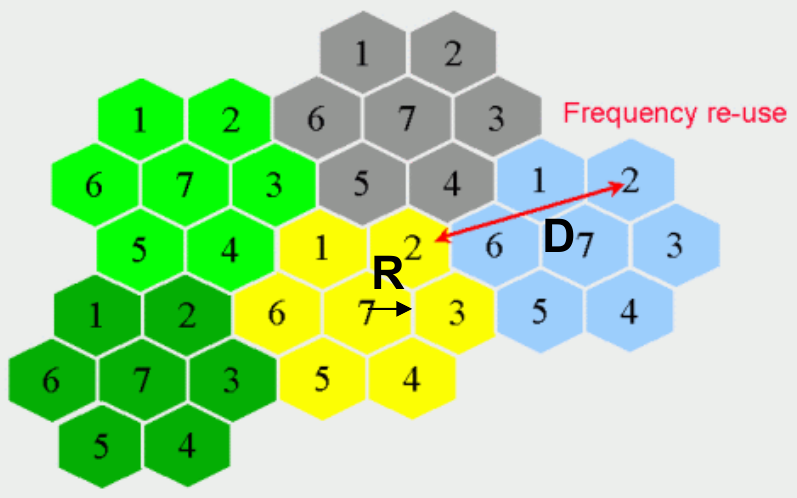
\includegraphics[
		width=10cm,
		%height=15cm
	]{images/Tema 4/Cellular systems description.png}
	\caption{
		\label{fig:unit4_cells_scheme}
		Cellular system scheme. The area is covered by clusters reusing the same frequencies.
	}
\end{figure}

\subsubsection{Interference}

To understand interference we can develope the following relations:

\begin{itemize}
	\item {
		Basic propagation losses:

		$$l_{b, c} = k \cdot R^n$$

		$$l_{b, i} = k (D - R)^n$$
	}
	\item {
		Received carrier signal:

		$$C = \frac {P_{tx}} {k \cdot R^n}$$
	}
	\item {
		Received interference:

		$$I = \frac {P_{tx}} {k (D - R)^n}$$
	}
	\item {
		Carrier-to-interference ratio:

		$$
			\left( \frac{C}{I} \right) = \left( \frac {D - R} {R} \right)^n \underset{\text{close to cell node}}{\approxeq} \left( \frac {D} {R} \right)^n
		$$
	}
\end{itemize}

If $R$ and $D$ are decreased, holding a given $\left( \frac{C}{I} \right)$, we can increase the reuse of frequencies and system capacity. However, $R$ is lower bounded by the protection rate:

$$
	\left( \frac{C}{I} \right) \ge r_p \rightarrow \left( \frac {D} {R} \right)^n \ge r_p
$$

We modeled a case in which a single co-channel cell was generating interference, but for $i_0$ co-channel cells surrounding the cell at the same distance, we would have:

$$
	I = \frac {i_0 \cdot P_{tx}} {k (D - R)^n} \rightarrow \left( \frac{C}{I} \right) = \frac{1}{i_0} \left( \frac {D - R} {R} \right)^n \underset{\text{close to cell node}}{\approxeq} \frac{1}{i_0} \left( \frac {D} {R} \right)^n
$$

\subsubsection{Dimensioning}

\begin{itemize}
	\item {
		\textbf{Traffic modeling}

		Mobile cellular systems are designed as blocking systems:

		$$
			GoS = P_B = \operatorname{B}(c, A_o)
		$$

		The offered traffic in a cell is:

		$$
			A_o = \operatorname{B}^{-1} (c, P_B)
		$$
		
		Where $\operatorname{B}^{-1}(\cdot)$ stands for Erlang B inverse function.

		Assuming that the median call duration is $s$ seconds and the mean number of calls at Busy Hour is $\lambda_{user}$, the offered traffic per user will be:

		$$
			a_o = s \cdot \frac {\lambda_{user}} {3600} [E]
		$$

		The number of mobile users in a cell is:

		$$
			m = \frac {A_o} {a_o}
		$$
	}
	\item {
		\textbf{Channelization}

		For the number of available channels:

		$$
			N_{cluster} = \frac {BW} {\Delta f} = \frac {BW} {f_{i} -  f_{i-1}}
		$$

		Where:
		\begin{itemize}
			\item $BW$: Available bandwidth for transmission or reception.
			\item $\Delta f$: Separation between radio frequency channels.
		\end{itemize}

		If the cluster has $J$ cells, the number of radiofrequency channels in a cell is:

		$$
			N_{cell} = \frac {N_{cluster}} {J}
		$$

		Usually, some radio frequency channels in the cell are reserved for signaling purposes:

		$$
			c = N_{cell} - N_{signaling}
		$$
	}
	\item {
		\textbf{Cell, cluster and coverage area dimensioning}

		The allowable \textbf{traffic intensity in the cell} is:

		$$
			\rho_a = \frac {A_o} {S_{cell}} [E / km^2]
		$$

		Where $S_{cell}$ is the cell area in $km^2$.

		Then, the area for the cluster is:

		$$
			S_{cluster} = J \cdot S_{cell}
		$$

		If the coverage area must be $S$, the number of clusters will be:

		$$
			Q = \operatorname{ceil} \left( \frac {S} {S_{cluster}} \right) + 1 \approxeq \frac {S} {J \cdot S_{cell}}
		$$

		$Q$ is also the number of times that frequencies are reused and it is called the \textbf{reuse factor}.

		The whole number of channels for traffic in the coverage area will be:

		$$
			N = Q \cdot J \cdot (N_{cell} - N_{signaling}) \approxeq N_{cluster} \cdot \frac {S} {J \cdot S_{cell}}
		$$

		And the total number of users will be:

		$$
			M = Q \cdot J \cdot m
		$$
	}
\end{itemize}

\subsubsection{Cellular geometry}

If in a cell, omnidirectional antennas are used, the coverage area will be approximately circular,
but circles do not cover the whole plane without overlapping.
Other polygons are used to cover the plane without overlapes,
there are three regular ones: triangle, square and hexagon.
The one with largest ratio area/radio is the hexagon, and so, it is used.

An inclined coordinated systems is used with a slope of 60 degrees.

\begin{figure}[H]
	\centering
	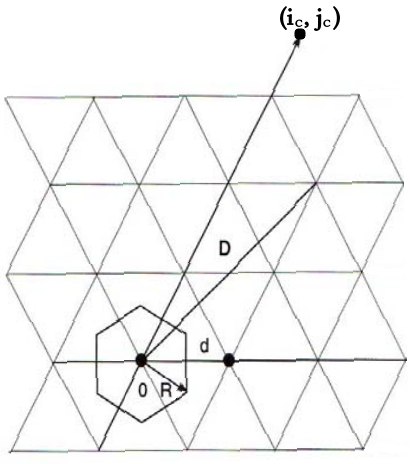
\includegraphics[
		width=9cm,
		%height=15cm
	]{images/Tema 4/Cellular geometry.png}
	\caption{
		\label{fig:unit4_cell_geometry}
		Cellular geometry
	}
\end{figure}

As a result of this design:
\begin{itemize}
	\item {
		Cells will have a radius $R$ related to cell area:

		$S_{cell} = \frac {3 \sqrt{3}}{2} R^2$
	}
	\item Having the node of a cell (geometrical center) at $(0, 0)$, we must select the coordinates of the node of the cell with the same frequency, the \textbf{co-channel node coordinates}: $i_c$, $j_c$
	\item The distance between the nodes of two neighboring cells will be the \textbf{lattice step} and will depend on co-channel node coordinates selected as well as the radius: $d = d(i_c, j_c) = R \cdot \sqrt{3}$
	\item {
		Each cell will be surrounded by 6 co-channel cells at \textbf{co-channel distance} $D$:

		$$
			i_0 = 6 \rightarrow I = \frac {6 \cdot P_{tx}} {k (D - R)^n} \rightarrow \left( \frac{C}{I} \right) = \frac{1}{6} \left( \frac {D - R} {R} \right)^n \underset{\text{close to cell node}}{\approxeq} \frac{1}{6} \left( \frac {D} {R} \right)^n
		$$
	}
	\item Only a limited set of natural numbers, known as \textbf{rhombic numbers} (1, 3, 4, 7, 9, 12, 13, 16, 19, 21, 25, 27, 28, 36, 37, 48, ...) can be given to the cluster size $J$ in order to avoid two co-channel cells face to each other.

\end{itemize}

Some useful relations are:
\begin{itemize}
	\item {
		Co-channel distance, lattice step, co-channel node coordinates and cluster size:

		$$
			D = d \cdot \sqrt{(i_{c}^2 + j_{c}^2 + i_{c} \cdot j_{c})} = d \cdot \sqrt{J}
		$$

		$$\updownarrow$$

		$$
			J = \left( \frac {D} {d} \right)^2 = i_{c}^2 + j_{c}^2 + i_{c} \cdot j_{c}
		$$

		$$\updownarrow$$

		$$
			d = \frac {D} {\sqrt{(i_{c}^2 + j_{c}^2 + i_{c} \cdot j_{c})}} = \frac{D}{\sqrt{J}}
		$$
	}
	\item {
		Co-channel distance, radius, co-channel node coordinates and cluster size:

		$$
			D = R \cdot \sqrt{3 (i_{c}^2 + j_{c}^2 + i_{c} \cdot j_{c})} = R \cdot \sqrt{3 J}
		$$

		$$\updownarrow$$

		$$
			J = \frac{1}{3} \left( \frac{D}{R} \right)^2 = i_{c}^2 + j_{c}^2 + i_{c} \cdot j_{c}
		$$

		$$\updownarrow$$

		$$
			R = \frac {D} {\sqrt{3 (i_{c}^2 + j_{c}^2 + i_{c} \cdot j_{c})}} = \frac{D}{\sqrt{3 J}}
		$$
	}
	\item {
		$J$ is lower bounded by protection rate:
		\begin{itemize}
			\item {
				Signal at the edge of the cell and interference at the center:

				$$
					\left( \frac{C}{I} \right) = \frac {1} {6} \left( \frac {D} {R} \right)^n \rightarrow
					J = \frac {1} {3} \left[ 6 \left( \frac{C}{I} \right) \right]^{\frac {2} {n}}
				$$

				$$
					\left( \frac{C}{I} \right) \geq r_p \rightarrow
					J \geq \frac {1} {3} \left( 6 r_p \right)^{\frac{2}{n}}
				$$
			}
			\item {
				Signal and interference at the edge:

				$$
					\left( \frac{C}{I} \right) = \frac {1} {6} \left( \frac {D - R} {R} \right)^n \rightarrow
					J = \frac {1} {3} \left( 1 + \left[ 6 \left( \frac{C}{I} \right) \right]^{\frac {1} {n}} \right)^2
				$$

				$$
					\left( \frac{C}{I} \right) \geq r_p \rightarrow
					J \geq \frac {1} {3} \left[ 1 + \left( 6 r_p \right)^{\frac{1}{n}} \right]^2
				$$
			}
		\end{itemize}
	}
	\item {
		Bit error rate for mobile problems:

		$$
			BER = \operatorname{Q} \left( \sqrt{2 \gamma \frac{E_b}{N_0}} \right)
		$$
	}
\end{itemize}

\subsubsection{Cellular division}

Cells can be divided into smaller ones according to demand (rural areas, urban areas, dense urban areas, etc.). It gives more flexibility to the planning process. The evolution is progressive. Dividing by two comes with:

\begin{itemize}
	\item Reduction in radio of the cell in half.
	\item Reduction of cell area by four.
	\item Increase in capacity approximately in four.
	\item BTS location must be more precise.
	\item The probability of handover is increased.
	\item Costs are increased.
\end{itemize}

\subsubsection{Sectoring}

Instead of using omnidirectional antennas at the very centre of each cell, directive antennas at the cell edges are used. In this way, the number of interference sources can be reduced due to antenna directivity.

Sectoring is carried out dividing the original cell into sectors that are covered by base stations at the alternate hexagon’s vertex.

\begin{figure}[H]
	\centering
	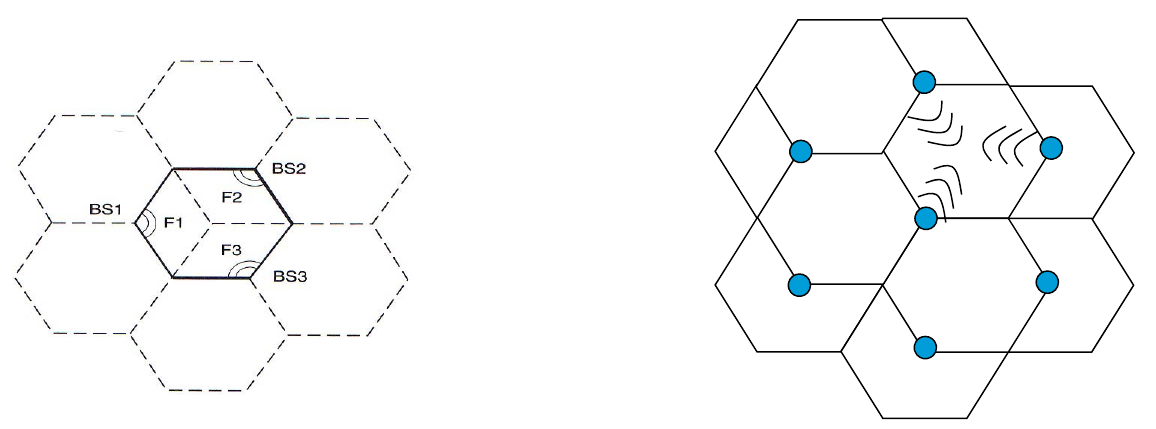
\includegraphics[
		width=14cm,
		%height=15cm
	]{images/Tema 4/Cellular sectoring 1.png}
	\caption{
		\label{fig:unit4_cell_sect_1}
		Cellular sectoring
	}
\end{figure}

This structure has some advantages:

\begin{itemize}
	\item The BTS can be supported by adjacent BTS cells, so we save in infrastructures.
	\item The co-channel interference is much lower due to the directivity of antennas.
	\item Thus, cluster size $J$ can be lower and then, the system capacity is higher due to the higher frequency reuse.
\end{itemize}

For example, if a cell is divided in two sectors, radius is reduced by half, surface is divided by four and capacity is multiplied by four.

Some drawbacks include:

\begin{itemize}
	\item Cost increment.
	\item BTS placement needs to be very precise.
	\item The probability of a hand-off increases.
\end{itemize}

\begin{figure}[H]
	\centering
	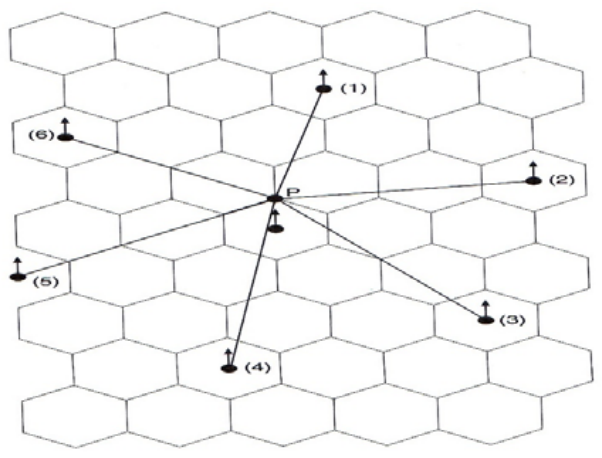
\includegraphics[
		width=7.5cm,
		%height=15cm
	]{images/Tema 4/Cellular sectoring 2.png}
	\caption{
		\label{fig:unit4_cell_sect_2}
		Cellular sectoring
	}
\end{figure}

\subsection{PMR and PMT systems}

Most widely used mobile communication systems can be classified as Private Mobile Radio (PMR) or Personal Mobile Telecommunications (PMT), and all the standards studied in this lesson belong to one of these categories.

\subsubsection{Private Mobile Radio / Professional Mobile Radio (PMR)}

A set of two-way radio systems. Usually not directly connected to public telephony network.

They are modeled as waiting systems:

$$
	GoS = \operatorname{P} \left( W_q > \frac{1}{\mu} \right) = \operatorname{C}(A_o, c) \cdot e^{- c \cdot \mu \cdot (1-\rho) \cdot t}
$$

The PMR main characteristics are:

\begin{itemize}
	\item Limited area (territorial).
	\item No usually directly connected to public switching telephony networks (PSTN)
	\item Fleet management. Enterprises.
	\item Example: TETRA (Trans European Trunked Radio)
\end{itemize}

Other characteristics:

\begin{itemize}
	\item MS to MS calls must be allowed.
	\item Calls are frequent and short in duration.
	\item Group calls must be permitted.
	\item Work in waiting regime, this is, they are modeled as waiting systems.
	\item Usually simplex (one or two frequencies) or semiduplex PTT (push to talk), although they can also be duplex.
\end{itemize}

Channel assignment:

\begin{itemize}
	\item Fixed assignment: the channel is fixed for a group of $M$ users that need to share it. It is simpler but lower performance. Used if the number of users is low.
	\item Trunked assignment: pool of $N$ channels being shared for $M$ users. More complex but much more efficient.
\end{itemize}

In case they use trunked assignment:

\begin{itemize}
	\item Pool of channels where the channel assignment is dynamic.
	\item They are waiting as the fixed assignment.
	\item A signaling protocol is needed for channel assignment and managing calling queues.
	\item In Europe, MPT 1327 protocol was developed in UK, which has been converted in fact the standard for such as systems. It is based on slotted ALOHA with variable frame length.
\end{itemize}

\subsubsection{Personal Mobile Telecommunications (PMT)}

Connected directly to public Telephony Network. Modeled as blocking systems. It is the public radio-telephony service, so it offers the mobile telephony service to the users. Any user, from a parked or moving vehicle, can sends or receive calls of/to any other fixed or mobile subscriber either national or international. These systems are, indeed, the PLMN (Public Land Mobile Network) with its own switching centers MSC (Mobile Switching Centers), that are connected to the public switched telephony service or other networks such as ISDN, data networks,

....

The main objectives are:
\begin{itemize}
	\item Large subscribers capacity to attend high traffic demands.
	\item Voice quality equal or higher than fixed service.
	\item Spectrum efficiency since we manage a limited number of frequencies, so frequency usage must be planned. The solution is frequency reuse by cellular planning.
	\item Radio frequency automatic switching.
	\item Capacity of expansion to achieve large coverage.
	\item Reasonable costs
\end{itemize}

Related concepts:
\begin{itemize}
	\item Handoff or handover: BS switching of a current voice call.
	\item Roaming: The mobile terminal moves from the own network to a different one.
	\item Downlink or direct channel: Radio channel for transmission from BS to MS (BS$\rightarrow$MS).
	\item Uplink or return channel: Radio channel for transmission from MS to BS (MS$\rightarrow$BS). Lower frequencies in the band are allocated to it.
\end{itemize}

\section{Terrestrial Trunking Radio (TETRA)}

It is the 2nd generation of standards for PMR systems in Europe. Among the facilities of TETRA we
have:

\begin{itemize}
	\item Duplex voice and data transmission.
	\item Data transmission up to 28.8 kbps.
	\item Optimized packet data transmission.
	\item Telemetry and slow video transmission.
	\item Communications security.
	\item Wide number of interfaces for interconnection with other networks.
	\item {
		Two modes:
		\begin{itemize}
			\item Voice + Data mode (V+D): Normal mode for telephony applications and data.
			\item Packet Data Optimized (PDO): It allows new data services such as e-mail, data interchange, location, ...
		\end{itemize}
	}
\end{itemize}

About radio interface:

\begin{itemize}
	\item {
		Basic radio interface specifications:
		\begin{itemize}
			\item 25 kHz channelization (optional 12.5 kHz).
			\item TDMA multiple-access with four intervals per frame.
			\item $\pi/4$ - DPSK modulation.
			\item Data rate 36 kbps.
			\item Protection rate of 19 dB.
		\end{itemize}
	}
	\item Within TDMA hierarchy. It uses a slot of 85/6 ms duration with capacity of 510 bits.
	\item Frame composed by four slot. Its duration is 56.67 ms.
	\item Multiframe composed by 18 frames. Its duration is 1.020 ms.
	\item Hiperframe composed by 60 multiframes.
\end{itemize}

\begin{tabular}{|c|c|c|c|c|}
	\hline
	Ramp	& Data		& Training		& Data		& Ramp \\
	\hline
	13 bits	& 216 bits	& 14+22+16 bits	& 216 bits	& 13 bits \\
	\hline
\end{tabular}

\section{Global System for Mobile Communications (GSM)}

\subsection{Introduction}

GSM is a mobile communications standard developed by ETSI. It is second generation communication system.

\subsection{Description}

\subsubsection{Services}

GSM attend a series of services:

\begin{itemize}
	\item {
		Basic Services:
		\begin{itemize}
			\item Bearer Services: Synchronous/Asynchronous transport capacity, packet or circuit mode at 9.600 bps.
			\item {
				Teleservices:
				\begin{itemize}
					\item Digital telephony with codec at total speed of 13 kbps or codec at half speed of 6.5 kbps.
					\item Short Messages Service (SMS).
					\item Facsimile: FAX Group 3.
				\end{itemize}
			}
		\end{itemize}
	}
	\item {
		Supplementary services:
		\begin{itemize}
			\item Calling line identification.
			\item Explicit call transfer.
			\item Waiting calls.
			\item Voice mail.
			\item Multi-party conferences.
			\item Billing (free calls, call collect, \ldots).
		\end{itemize}
	}
\end{itemize}

\subsubsection{Characteristics}

GSM main characteristics are:

\begin{itemize}
	\item It uses GMSK modulation.
	\item {
		Protection co-channel rate:

		$$
			R_p = 9 [dB]
		$$

		$$
			\left( \frac{S}{I} \right) = \frac {(\sqrt{3 J})^n} {i_o}
		$$

		$$
			\left( \frac{S}{I} \right)_{dB} = 10 \log \left( \frac {(\sqrt{3 J})^n} {i_o} \right)
		$$

		As we saw, $i_o$, the number of sides of the cell, will be typically 6, resulting in previous expressions.
	}
	\item Channel bandwidth: 200 kHz 8 channels/carrier
	\item Doppler distortion: Up to 200 km/h can be compensated.
	\item Temporal distortion: Up to 16 $\mu$s can be equalized.
	\item Cellular structure: Sectored in urban areas and omnidirectional in rural areas.
	\item Multiple-Access: TDMA with 8 intervals per frame (8 physical channels per carrier frequency).
	\item Frequency Hopping (FH): Mobile Subscriber (MS) can change the frequency from frame to frame (217 hops per second) in order to avoid the multipath fading.
	\item Discontinuous Tx (DTX): Data is only sent when user is talking, otherwise, comfort noise is generated at receiver.
	\item Security: Communications are ciphered and access system authentication is required.
	\item {
		Frequency bands for GSM-900 in its P version (most extended one) are:
		\begin{itemize}
			\item MS-BS link: 890 - 915 MHz (25 MHz).
			\item BS-MS link: 935 - 960 MHz (25 MHz).
		\end{itemize}
		These bands are divided into 124 pairs separated 200 kHz each other:

		$f_{MS-BS} = 890.2 + 0.2 \cdot (n - 1) [MHz]$

		$f_{BS-MS} = f_{MS-BS} + 45 [MHz] = 935.2 + 0.2 \cdot (n - 1) [MHz]$

		$n = 0, 1, 2, \ldots, 125$
	}
	\item {
		Frequency bands for GSM-DCS-1800 are:
		\begin{itemize}
			\item Uplink: 1710 - 1785 MHz (75 MHz).
			\item Downlink: 1805 - 1880 MHz (75 MHz).
		\end{itemize}
	}
\end{itemize}

\subsubsection{Mobile Subscriber (MS) identification}

In order to identify and manage Mobile Subscribers (MS), GSM defines the following information fields:

\begin{itemize}
	\item International Mobile Equipment Identity (IMEI): It identifies the terminal and is burnt by manufacturer.
	\item International Mobile Subscriber Identity (IMSI): It identifies the user internationally. It is associated to SIM card. IMSI is not known by the user, except spoiler. It is used by the network for authentication and call establishment. It is used the first time (GSM attach) and then it is changed to a temporal one (TMSI), assigned by a device called VLR.
	\item Temporal Mobile Subscriber Identity (TMSI): Temporal mobile subscriber identity assigned by VLR.
	\item {
		Mobile Station ISDN (MS-ISDN): It is the user telephone number. It follows the format:

		\texttt{CC (country) | NDC (operator prefix) | Subscriber number}
	}
	\item Mobile Subscriber Roaming Number (MSRN): It is another number used for routing.
\end{itemize}

\subsection{Architecture}

\subsubsection{Elements}

GSM architecture is implemented through the following elements:

\begin{itemize}
	\item Public Switching Telephony Network (PSTN).
	\item Mobile Switching Center (MSC): It manages calls from or to MS and establishes conections with other networks (PSTN, ISDN, \ldots).
	\item Home Location Register (HLR): It is the whole subscriber register. It stores IMSI, MSISDN, location information, \ldots
	\item Visitors Location Register (VLR): It is the visiting subscribers register for temporal users controlled by the MSC. It stores IMSI, TMSI, MSRN and a copy of profile data from HLR for users.
	\item Base Station Controller (BSC): Most functions are at the BSC, allowing BTS being very simple.
	\item Base Transceiver Station (BTS).
	\item Mobile Terminal (MT).
	\item Terminal Equipment (TE).
	\item Authentication Center (AUC): It is the authentication center. It stores identity information for users to verify calls and users.
	\item Equipment Identity Register (EIR).
	\item Operation and Maintenance Center (OMC).
	\item Network Management Center (NMC).
	\item Administration Center (ADC).
	\item Operation Subsystem (OSS).
	\item Base Station Subsystem (BSS).
	\item Mobile Station (MS).
\end{itemize}

\subsubsection{Interfaces}

Two main interfaces have been defined:

\begin{itemize}
	\item Line interface (A): It separates the switching center (MSC) and the base station subsystem (BSS). There is also an optional interface (A-bis) between the BSC and BTS.
	\item Radio interface (Um): It places the borderline between base stations and mobile terminals (MS).
\end{itemize}

\subsubsection{Scheme}

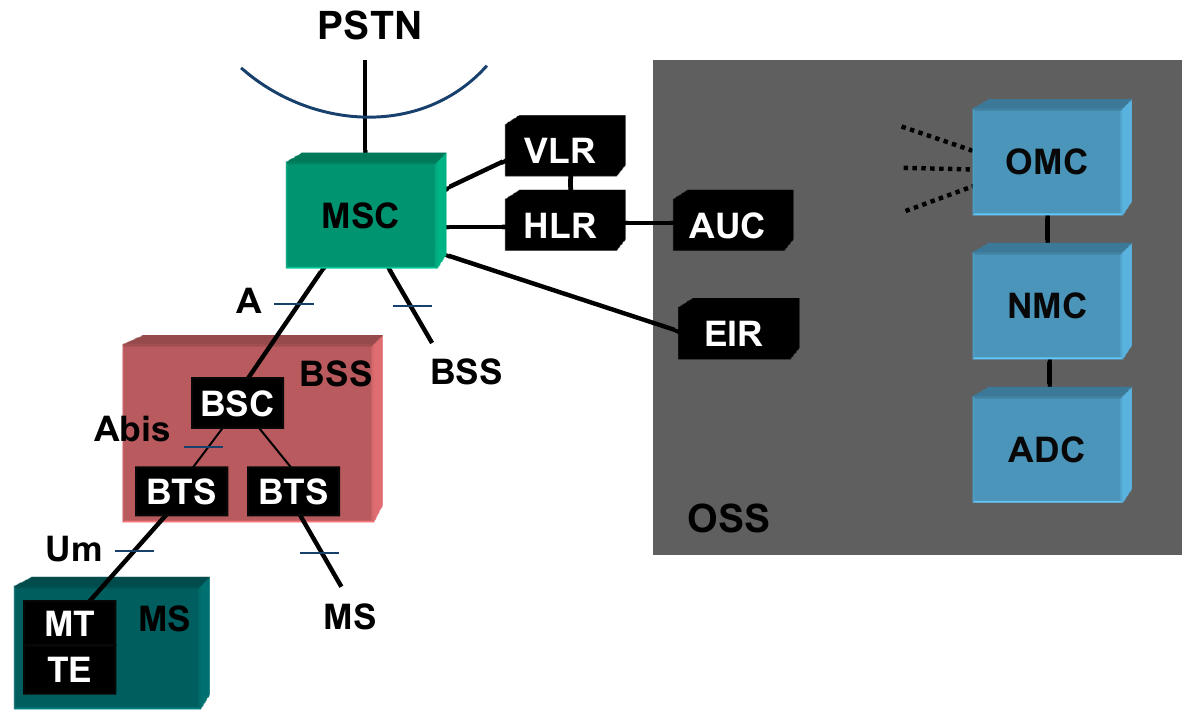
\includegraphics[
	width=10cm,
	%height=15cm
]{images/Tema 4/GSM architecture.png}

\subsection{GSM frame}

\subsubsection{Frame structure}

Each GSM frame is composed by 8 time-slots. The frame duration is 4,615 ms and thus, each time-slot is lasts 0,577 ms. This structure is for uplink and downlink, but with a delay of 3 time-slots. In this way, a mobile transmits or receives, but not both simultaneously.

\begin{figure}[H]
	\centering
	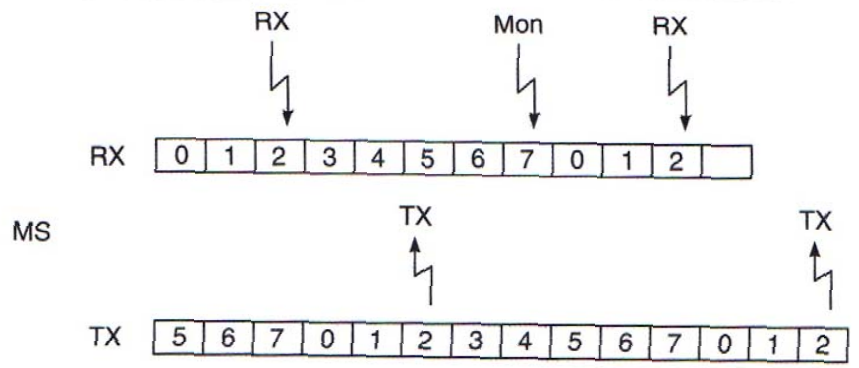
\includegraphics[
		width=7cm,
		%height=15cm
	]{images/Tema 4/GSM frame.png}
	\caption{
		\label{fig:unit4_GSM_frame}
		GSM frame
	}
\end{figure}

\subsubsection{Burst}

Data information is sent inside the time-slot in a burst of bits. Each burst has 148 bits. At the end of the burst, the time equivalent of 8.25 bits is appended as guard period. Thus, the data rate at the radio interface is:

$$
	\frac {156.25 [b]} {0.577 [ms]} = 270.833 [kbps]
$$

There are several types of burst:
\begin{itemize}
	\item Normal burst.
	\item Frequency correction burst.
	\item Synchronization burst.
	\item Dummy burst.
	\item Access burst.
\end{itemize}

Normal burst has 148 bits and the guard period (156.25 bits in total):
\begin{itemize}
	\item Tail Bits (TB): 3+3 bits of header (one header for each data bits set).
	\item Data bits: 2 x (57 bits + 1 bit) = 116 bits. Two sets of data bits. The 57 bits part is information, and the other bit is a flag to indicate if is TCH or FACCH.
	\item Training Sequence (TS): 26 bits. Used for channel estimation and adjusting the equalizer.
	\item Guard Period (GP): Time equivalent to 8.25 bits.
\end{itemize}

\begin{tabular}{|c|c|c|c|c|c|}
	\hline
	TB 1 (3 bits)	& Data 1 (58 bits)	& TS (26 bits)	& Data 1 (58 bits)	& TB 2 (3 bits)	& GP (8.25 bits) \\
	\hline
\end{tabular}

\subsubsection{Hierarchy}

The frame hierarchy can be visualized in the following picture:

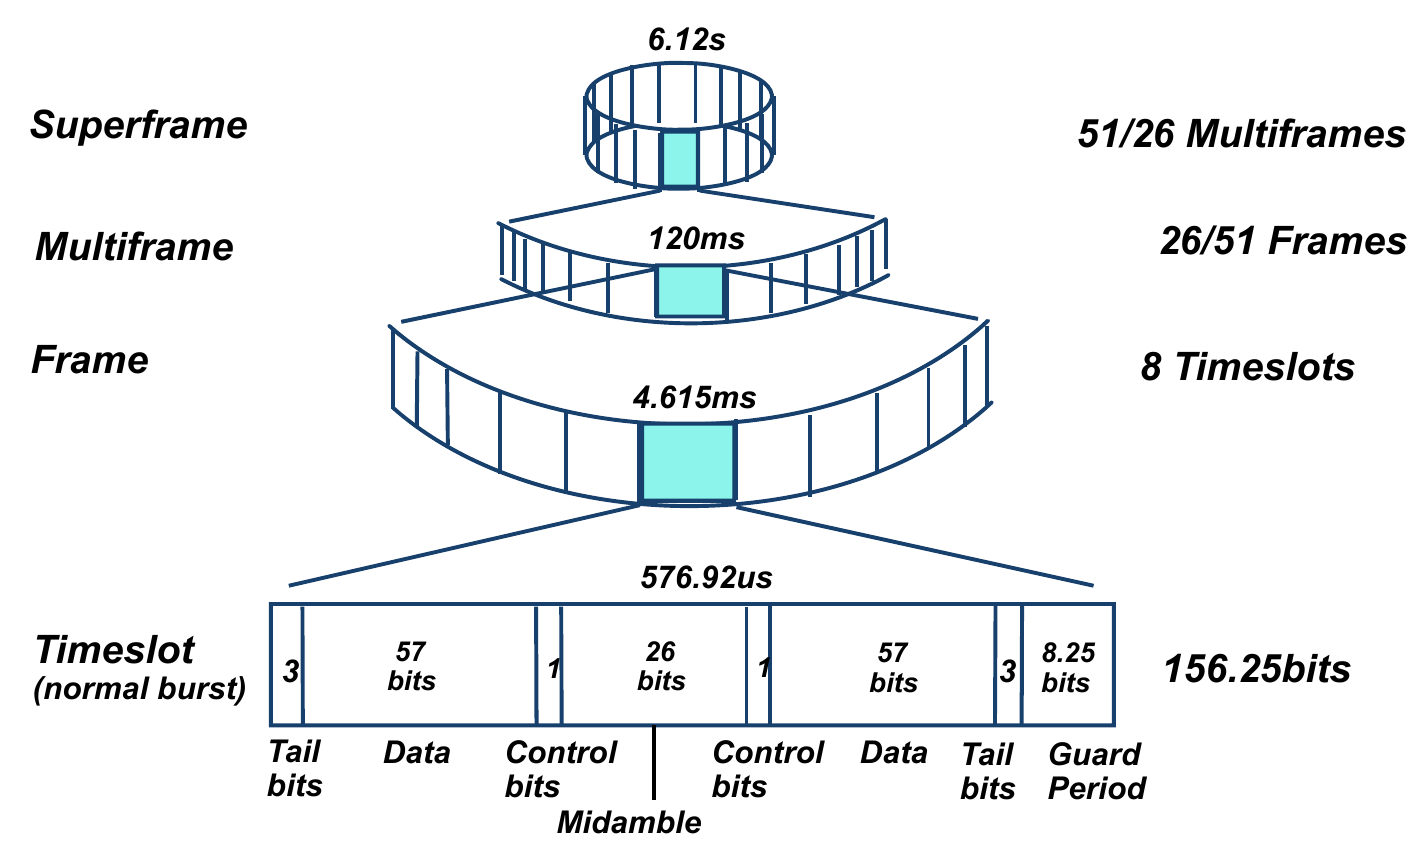
\includegraphics[
	width=12cm,
	%height=15cm
]{images/Tema 4/GSM frame hierarchy.png}

\subsection{Logical channels}

GSM establishes a set of logical channels.

\subsubsection{Traffic channels (TCH)}

They are mapped onto a pair of subcarriers and slots. There are seven types for these channels:
\begin{itemize}
	\item Full rate voice (TCH/F).
	\item Half rate voice (TCH/H).
	\item Data at speed of 2.4, 4.8 and 9.6 kbps.
	\item Data at half speed of 2.4 and 4.8 kbps.
\end{itemize}

In each communication, each traffic channel has a signaling channel associated to control the call:
\begin{itemize}
	\item Slow Associated Control Channel (SACCH): Common signaling associated to the voice call such as power control, billing, timing advanced, quality, \ldots
	\item Fast Associated Control Channel (FACCH): Urgent signaling such as in handovers. It steals bits to the traffic channel.
\end{itemize}

\subsubsection{Signaling channels}

\begin{itemize}
	\item {
		Broadcast channels: They work in the downlink and they are intended for all the terminals. They are supposed to help in synchronization, for example:
		\begin{itemize}
			\item Broadcast Control Channel (BCCH): General cell information and network.
			\item Frequency Correction Channel (FCCH): It is used for frequency acquisition by the MS.
			\item Synchronization Channel (SCH): It is used for synchronization and BS identification purposes.
		\end{itemize}
	}
	\item {
		Common control channels (CCCH): They are used to control the access to the network from terminals. They are uplink and downlink. They are:
		\begin{itemize}
			\item Ramdom Access Channel (RACH): Uplink. MSs request the access to the network (e.g., originated call). Slotted ALOHA is used.
			\item Paging Channel (PCH): Downlink. The network notifies to MS about incoming calls or messages.
			\item Access Grant Channel (AGCH): Downlink. Resource assignments.
		\end{itemize}
	}
	\item {
		Dedicated control channels: Bidirectional channels dedicated between a MS and the network. Previous to a call transmission:
		\begin{itemize}
			\item Stand-alone Dedicated Control Channel (SDCCH): Divided into 8 channels (D0, D1, \ldots, D7), each one is associated to one MS for signaling purposes.
			\item Slow Associated Control Channel (SACCH): It is the associated control channel for the SDCCH. It is also divided into 8 channels A0, A1, \ldots, A7, associated to D0, D1, \ldots, D7.
			\item Fast Associated Control Channel (FACCH).
		\end{itemize}
		The set Dn/An is usually denoted as SDCCH/8.
	}
\end{itemize}

\begin{figure}[H]
	\centering
	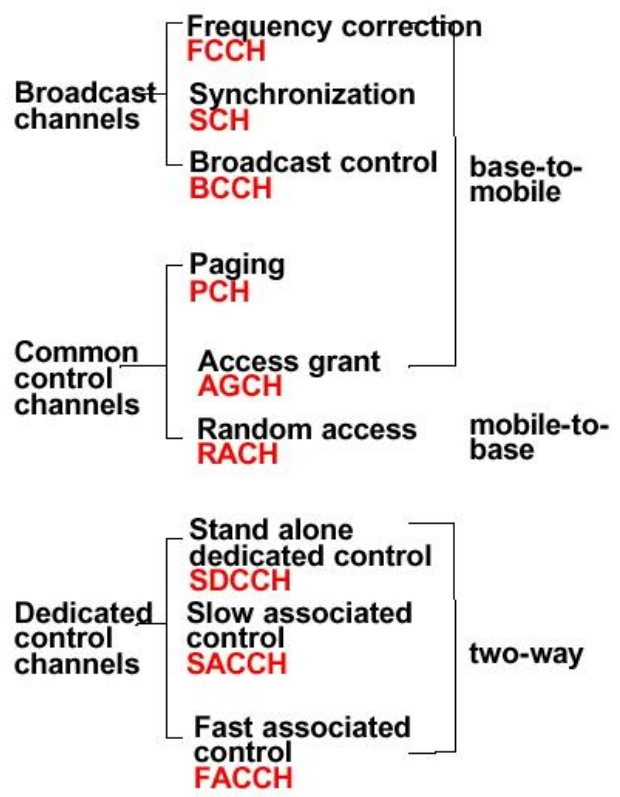
\includegraphics[
		width=7cm,
		%height=15cm
	]{images/Tema 4/GSM logical channels.png}
	\caption{
		\label{fig:unit4_GSM_log_channels}
		GSM logical channels
	}
\end{figure}

\subsection{Implementation of services}

\subsubsection{Voice encoding process}

The vocoder used in GSM is Regular Pulse Excited-Long Term Prediction (RPE-LTP). It produces 260 bits each 20 ms (i.e., 13 kbps). The 260 bits are classified into three categories, 1a, 1b and 2, according to their importance and sensitivity to errors.

The process consists in:
\begin{itemize}
	\item There are 50 type 1a bits. They are encoded by using a block code ($53, 50$) and so we get 53 bits ($50 \rightarrow 53$).
	\item To those former 53 bits, the 132 bits from the class 1b and a tail of 4 bits are appended ($53 \rightarrow 189$).
	\item The resultant 189 bits are encoded by a 1/2 convolutional code of length 5 to get 378 bits ($189 \rightarrow 378$).
	\item Finally, the other 78 bits from class 2 are added obtaining the final 456 bits of the frame ($378 \rightarrow 456$).
	\item These 456 bits are transmitted into 8 blocks of 57 bits, and thus, 8 sub-slots from 4 consecutive frames are needed to transmit them ($456 = 8 \cdot 57$ $\rightarrow$ 8 sub-slots $\rightarrow$ 4 frames).
\end{itemize}

\subsubsection{Mobility management}

Two kind of management are needed:
\begin{itemize}
	\item When the terminal is attached to the network but without conversation. Only the update of MS location is needed for future calls.
	\item When the terminal is currently in a voice call. Besides location, radio frequency switching are needed in handovers.
\end{itemize}

\subsubsection{Security}

The following aspects are involved into GSM security:
\begin{itemize}
	\item Subscriber identity authentication.
	\item Subscriber identity confidentiality.
	\item Control signaling confidentiality.
	\item Subscriber data confidentiality.
\end{itemize}

The subscriber is uniquely identified by using the IMSI jointly with the authentication subscriber's key ($K_i$).

The $K_i$ is never sent through the air in clear. There is a challenge-response mechanism for authentication. The BS sends a random number of 128 bits (RAND). The MS calculates the signed response of 32 bits (SRES) with the RAND and the $K_i$ based on the A3 algorithm.

The network does the same. If both SRES are the same, the subscriber is authenticated. The $K_i$ never outs form SIM and the IMSI only once (the first time).

\section{Universal Mobile Telecommunications System (UMTS)}

\subsection{Introduction}

UMTS is the evolution of GSM and belongs to third generation of mobile communication systems. The road from GSM to UMTS includes some intergenerational communication systems:
\begin{itemize}
	\item {
		High Speed Circuit Switched Data (HSCSD):
		\begin{itemize}
			\item Data transfer same as GSM but with many slots.
			\item Circuit switched
			\item Problems with terminals delayed the launching.
		\end{itemize}
	}
	\item {
		Global Packet Radio Service (GPRS):
		\begin{itemize}
			\item Packet based radio access and IP backboned. When a user sends data, they are encapsulated into short packets, with a header with source and destination. Each packet can follow different paths. Whereas GSM was defined for voice, the main objective of GPRS is to offer data packet such as TCP/IP.
			\item GPRS only use network resources when data need to be transmitted/received.
			\item GPRS reuse GSM’s architecture and infrastructure.
			\item {
				New elements are added for packet switching:
				\begin{itemize}
					\item Serving GPRS Support Node (SGSN).
					\item Gateway GSN Support Node (GGSN): It is the gateway among GPRS network an the other networks, including other GPRS networks from other operators.
					\item Gateway MSC (GMSC).
				\end{itemize}
			}
			\item Different mobile classes (capacity from 1 to 8 slots).
			\item Speed: 144 kbps (very low).
		\end{itemize}

		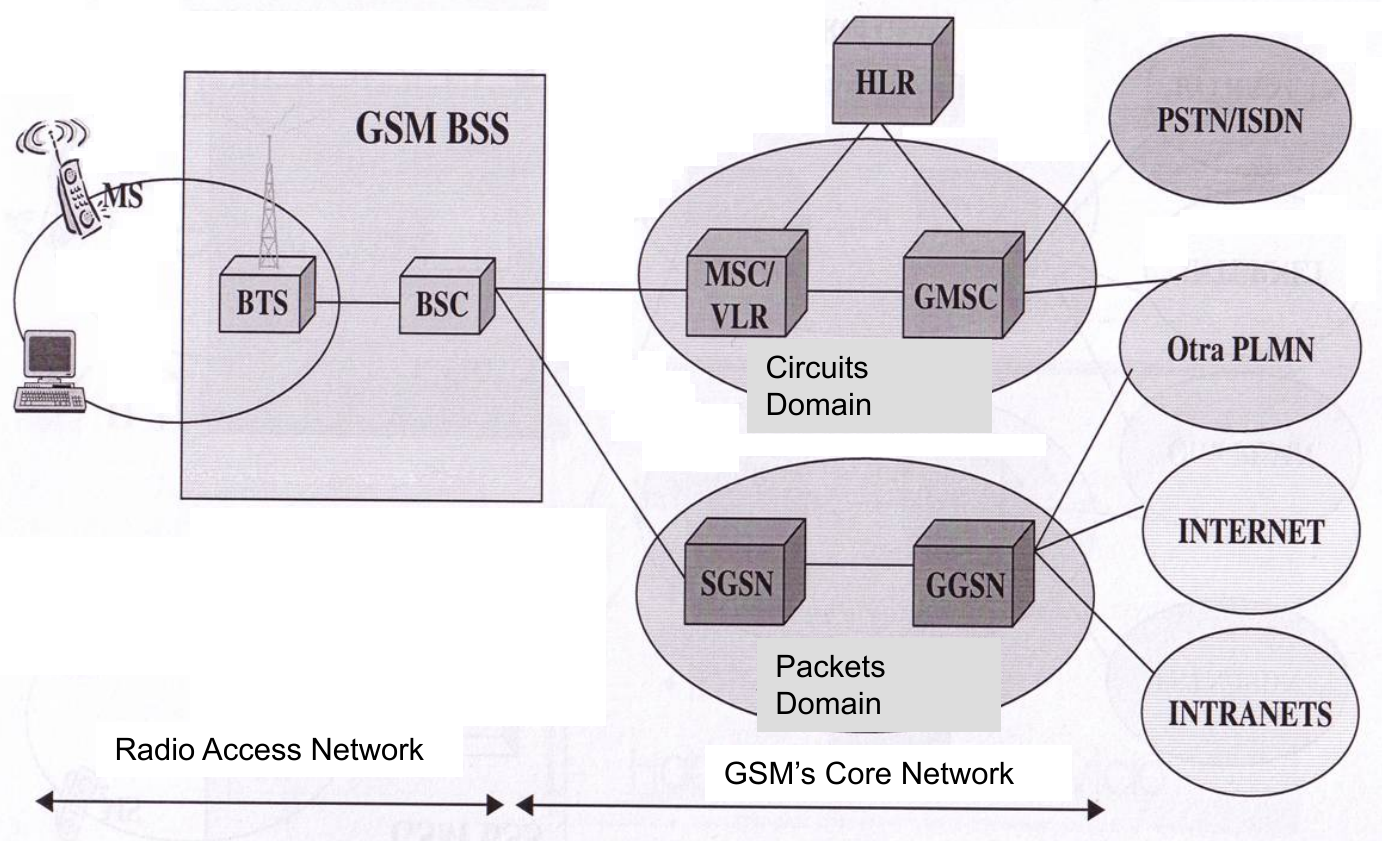
\includegraphics[
			width=10cm,
			%height=15cm
		]{images/Tema 4/GPRS architecture.png}
	}
	\item {
		Enhanced Data rate for Global Evolution (EDGE):
		\begin{itemize}
			\item New 8PSK modulation.
			\item Evolution of GPRS with adaptive modulation and coding (AMC).
			\item High hardware impact on terminals and BTS with respect to GPRS.
			\item Speed up to 384 kbps.
			\item Low market interest.
		\end{itemize}
	}
	\item {
		EDGE Evolution:
		\begin{itemize}
			\item High market acceptance.
			\item Up to 1 Mbps.
			\item Up to 32 QAM and 10 TS (two carriers).
			\item Two antennas.
			\item Turbo codes.
		\end{itemize}
	}
\end{itemize}

UMTS is developed by 3rd Generation Parthership Project (3GPP), which generates UMTS specifications. It is composed by standardization organisms worldwide:
\begin{itemize}
	\item ETSI (Europe).
	\item ARIB, TTC (Japan).
	\item T1 (USA).
	\item CWTS (China).
\end{itemize}

It is not a normalization organism because it does not have legal attributions, but it is composed by those organism that own the legal attributions such as ETSI in Europe.

\subsection{Specifications}

UMTS seeks to achieve better specifications:
\begin{itemize}
	\item Higher capacity for basic services (voice).
	\item {
		New data and multimedia services:
		\begin{itemize}
			\item 144 kbps (rural environments, total mobility).
			\item 348 kbps (urban environments, limited mobility).
			\item 2 Mbps (indoors).
		\end{itemize}
	}
	\item Packets technology and IP protocols (Internet)
	\item More roaming.
	\item Reconfigurable terminals and capacity of downloading services and applications.
\end{itemize}

\subsection{Architecture}

UMTS network is composed by the following elements:
\begin{itemize}
	\item {
		Core network: It transports information, both traffic and signaling. It owns the system intelligent (routing, control, mobility management, \ldots). It is connected to other networks. It is an evolution from GPRS/GSM core network, so the same elements are present:
		\begin{itemize}
			\item HLR, VLR, AuC, EIR and SMS centers.
			\item Circuit Switched elements: MSC and GMSC, that are denoted as U-MSC and U-GMSC.
			\item Packet Switched elements: SGSN and GGSN, that are denoted U-SGSN and U-GGSN.
		\end{itemize}
		The separation between packet and circuit switching is needed because of the evolution from former networks, although the trend is the single network ``all IP-based''.
	}
	\item {
		UMTS Terrestrial Radio Access Network (UTRAN):
		\begin{itemize}
			\item {
				Similar architecture as in GSM, although functionalities changes:
				\begin{itemize}
					\item BTS $\rightarrow$ Node B.
					\item BSC $\rightarrow$ Radio Network Controller (RNC).
				\end{itemize}
			}
			\item {
				A new normalized interface (Iur) between RNCs has been defined. Radio access technology is CDMA:
				\begin{itemize}
					\item Spread spectrum technique (5 MHz) instead of narrowband GMSK signal of GSM.
					\item All users in a cell share the same bandwidth but with different codes.
				\end{itemize}
			}
			\item FDD (typical) and TDD (hot-spot) have been defined.
			\item There is also an element called Radio Network System (RNS).
		\end{itemize}
		\begin{figure}[H]
			\centering
			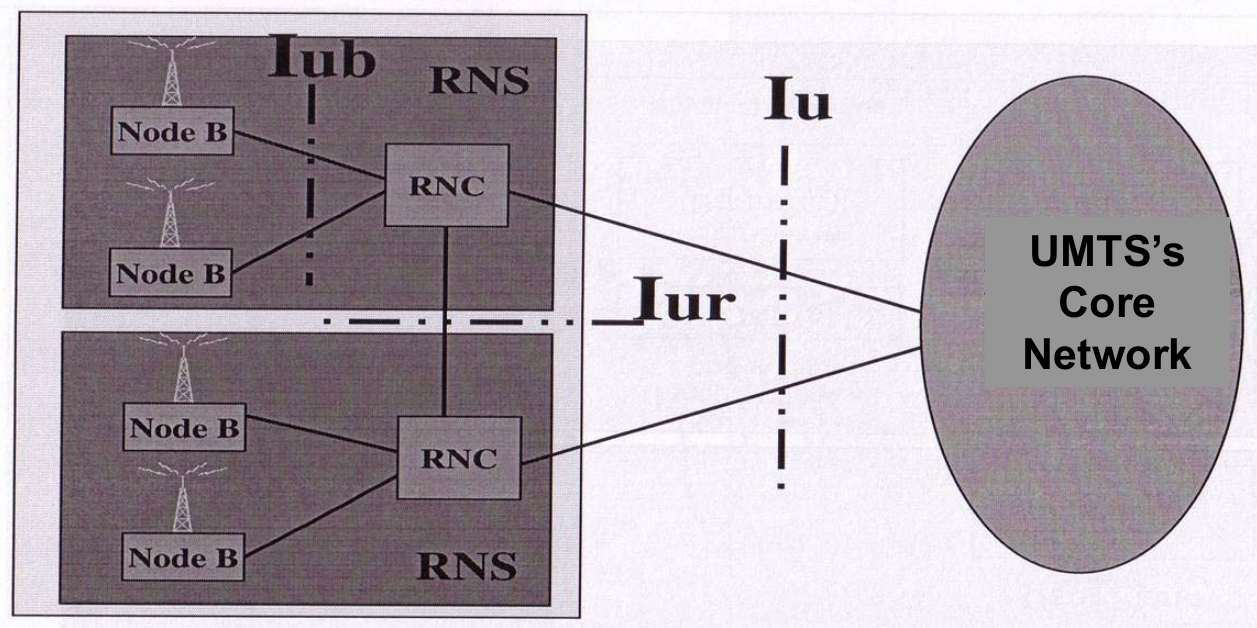
\includegraphics[
				width=10cm,
				%height=15cm
			]{images/Tema 4/UTRAN.png}
			\caption{
				\label{fig:unit4_UTRAN_arch}
				UTRAN architecture
			}
		\end{figure}
	}
	\item User Equipment (UE): It is the mobile terminal and the identification element (SIM equivalent for UMTS).
\end{itemize}

\begin{figure}[H]
	\centering
	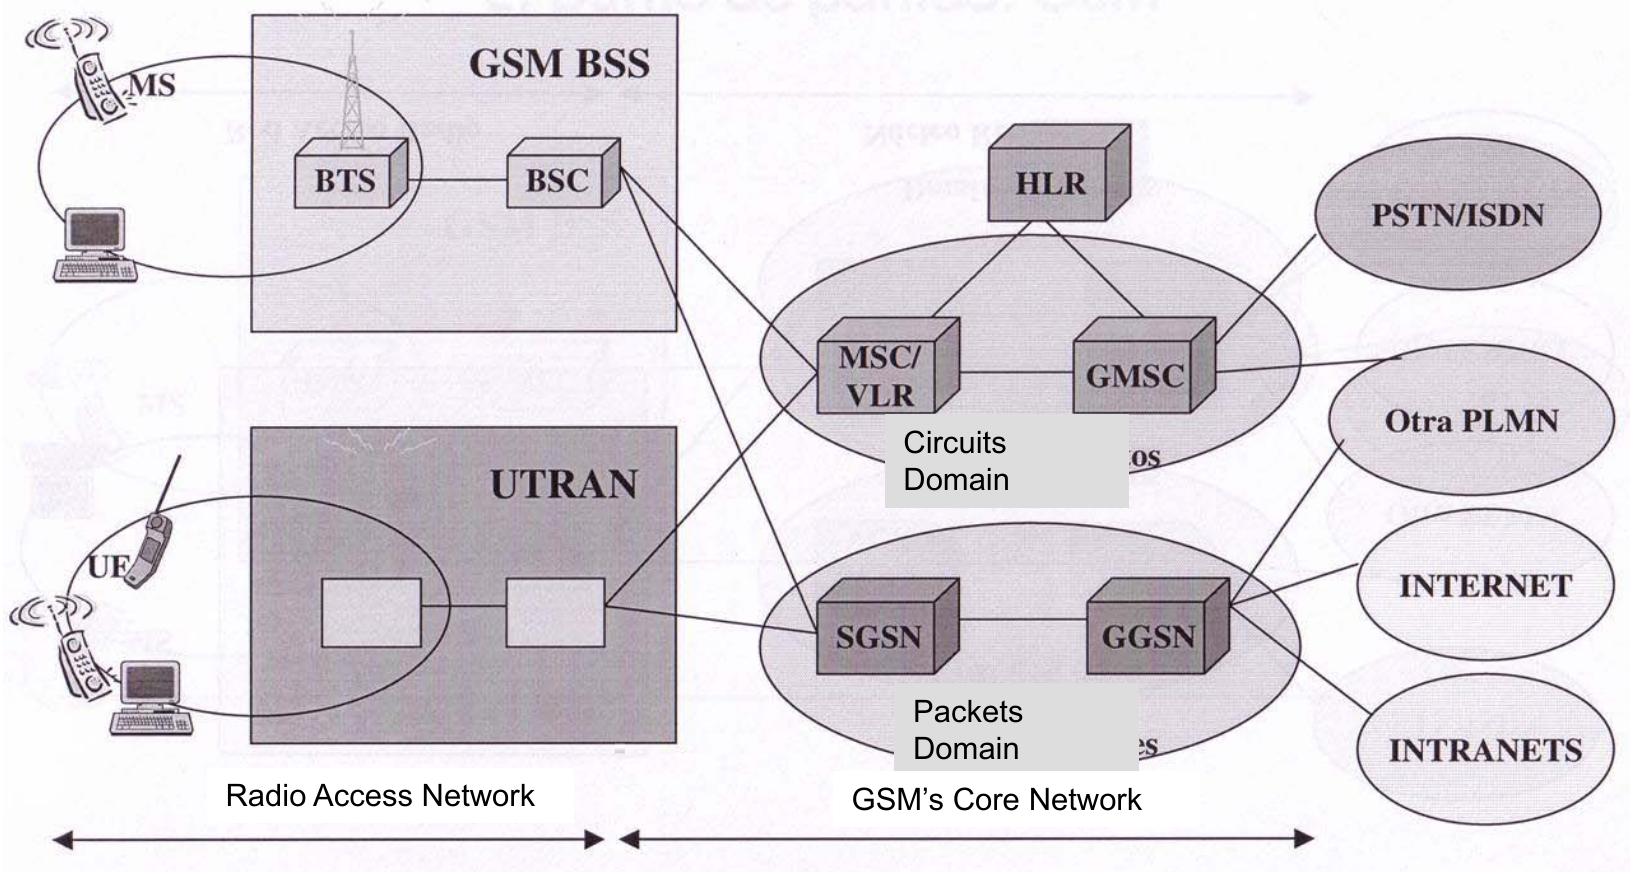
\includegraphics[
		width=14cm,
		%height=15cm
	]{images/Tema 4/UMTS architecture.png}
	\caption{
		\label{fig:unit4_UMTS_arch}
		UMTS architecture
	}
\end{figure}

\section{High Speed Downlink Packet Access (HSDPA)}

\subsection{Introduction}

HSDPA is the evolution of 3G from WCDMA that allows higher data rates in the downlink. It theoretically allows data rates of up to 14 Mbit/s. In practice, it is limited to 10,7 Mbits/s. It allows to reduce the data services latency, which was one of the main weakness in GPRS and WCDMA.

\subsection{Description}

HDSPA includes two groups of technical improvements:

\begin{itemize}
	\item {
		New scheme for the radio resources management: Instead of controlling the transmission power to guarantee a constant bit rate, the power is kept constant and the data rate is maximized to this power.

		\begin{figure}[H]
			\centering
			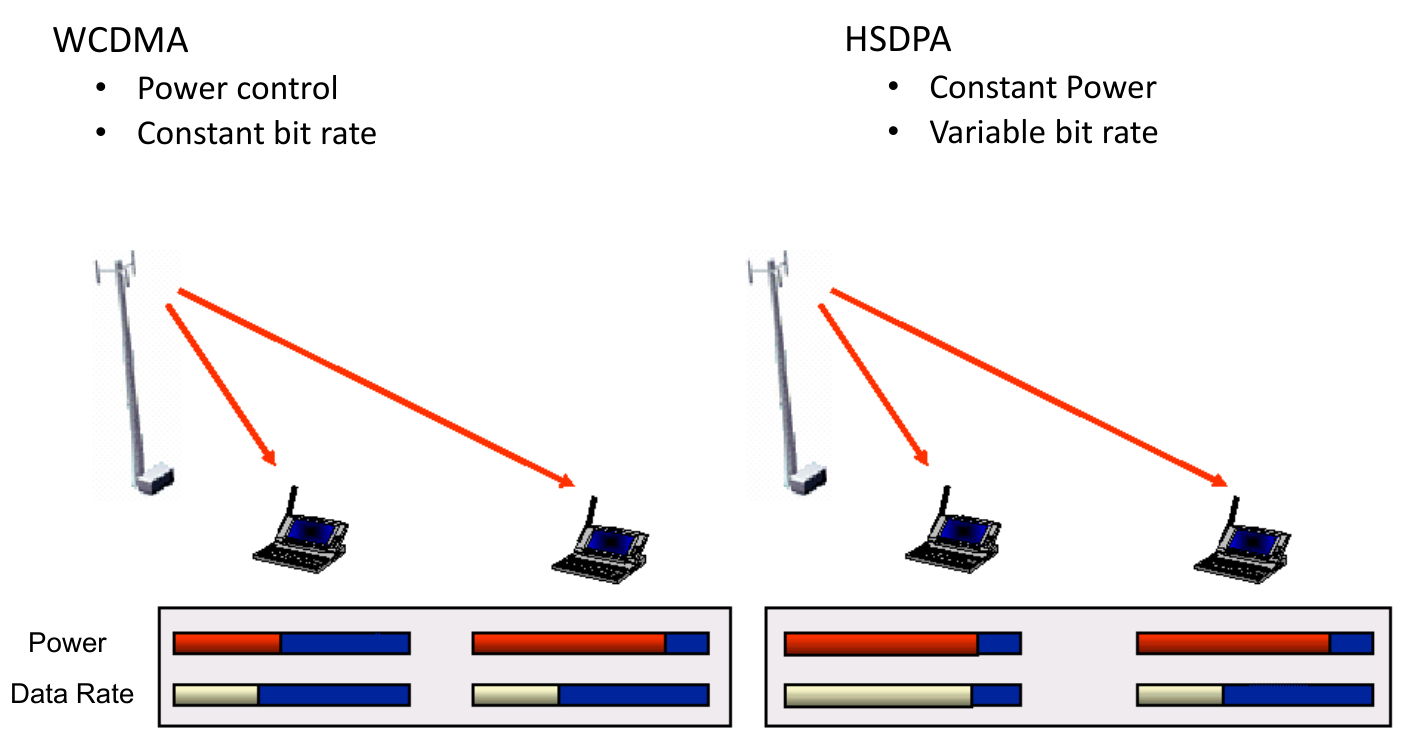
\includegraphics[
				width=14cm,
				%height=15cm
			]{images/Tema 4/WCDMA vs HDSPA.png}
			\caption{
				\label{fig:unit4_WCDMA_HDSPA}
				WCDMA vs HDSPA
			}
		\end{figure}
	}
	\item {
		New technologies supporting higher data rates:
		\begin{itemize}
			\item {
				Adaptive Modulation and Coding (AMC): The modulation and coding scheme is selected according to the current propagation quality in order to maximize the bit rate constraint to the bit error rate.

				\begin{figure}[H]
					\centering
					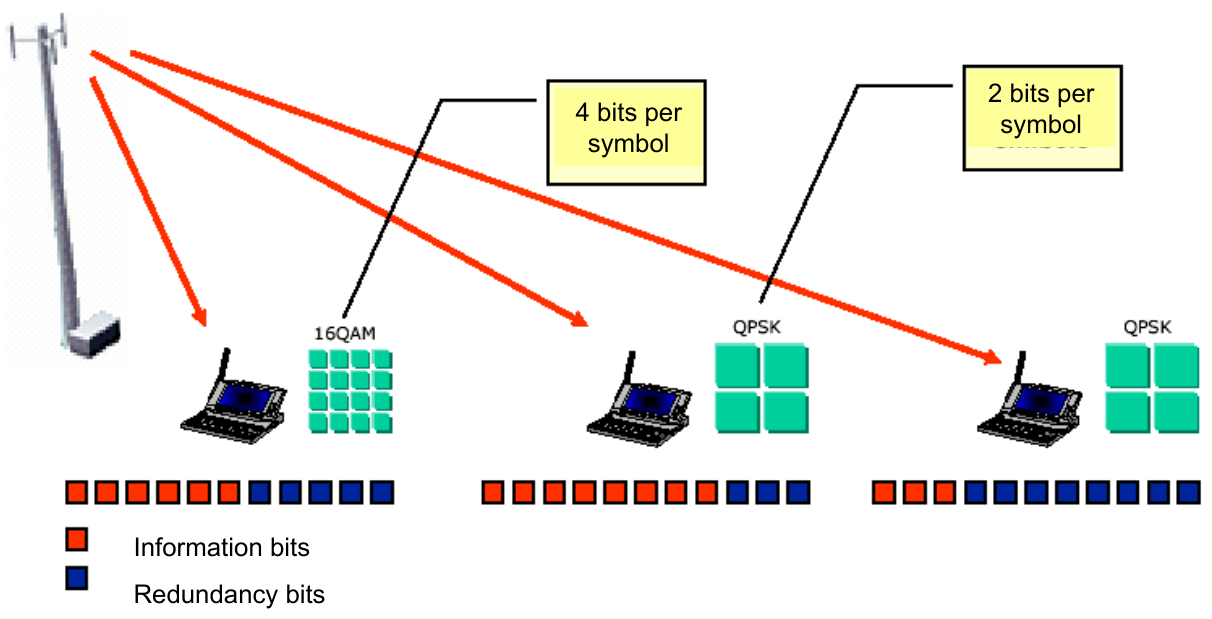
\includegraphics[
						width=14cm,
						%height=15cm
					]{images/Tema 4/HSDPA modulation and coding.png}
					\caption{
						\label{fig:unit4_HDSPA_mod_cod}
						HSDPA modulation and coding
					}
				\end{figure}
			}
			\item {
				Fast resources assignment: Resources are given to the terminal with the best channel quality at any moment, so the terminal that is transmitting can have the highest data rate. The gain is larger when channels from different users are uncorrelated or the number of users increases.

				\begin{figure}[H]
					\centering
					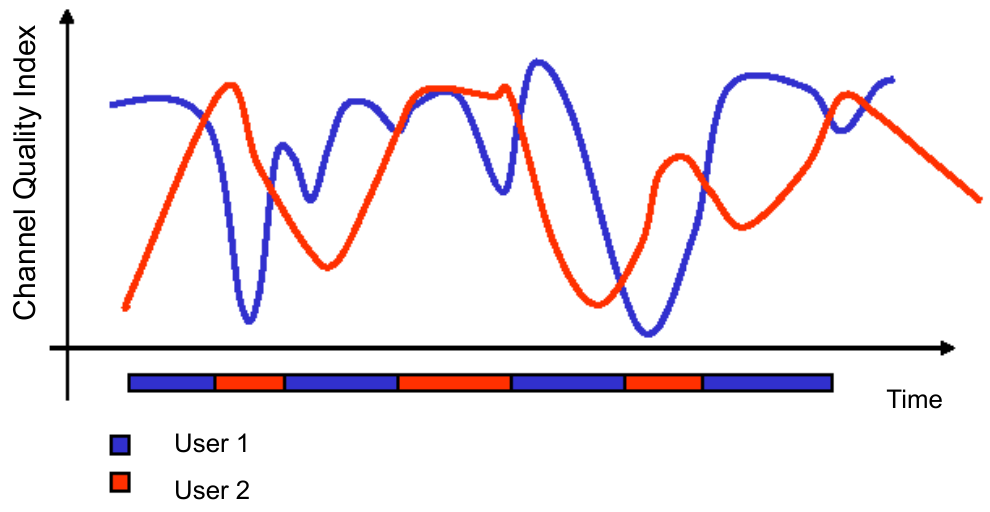
\includegraphics[
						width=14cm,
						%height=15cm
					]{images/Tema 4/HSDPA resources assignment.png}
					\caption{
						\label{fig:unit4_HDSPA_resources}
						HSDPA resources assignment
					}
				\end{figure}
			}
			\item {
				Hybrid Request Mechanisms (H-ARQ): Optimization of request mechanisms in case of retransmissions. Hybrid system is implemented with two methods:
				\begin{itemize}
					\item Chase combination (simple redundancy): The idea is to keep all the packets retransmissions and try the decoding process by combining all of them with different weights according to their SNR. This methods gets diversity gain and it is very simple to implement. Transmitter is not modified (retransmissions are the same).
					\item {
						Incremental redundancy (IR): Instead of retransmitting the same, different redundancy data is sent in each retransmission. For example:
						\begin{itemize}
							\item We use a turbo code of 1/3 and 2/3 of information is deleted (punctured). Data rate is then 1 (iqual to information rate).
							\item At the receiver side, punctured bits are restored and decoding is performed.
							\item If the decoding process fails, the retransmission includes new redundancy bits different from previous transmission.
							\item If receiver still has the previous packet, now it will have 2/3 information bits. Successful decoding probability increases in this iteration.
							\item The process continues until the packet is successfully decoded.
						\end{itemize}
					}
				\end{itemize}
			}
		\end{itemize}
	}
\end{itemize}

\subsection{HSPA+}

Its a dual cell or dual carrier HSDPA, this is, two 5 MHz carriers simultaneously. Carrier aggregation is implemented in order to improve spectral efficiency and allowing load balance between carriers.

We get higher data rates:
\begin{itemize}
	\item At uplink, up to 23 Mbps.
	\item At downlink, up to 84 Mbps.
\end{itemize}

The specifications for HSPA uplink and downlink are in 25 series from 3GPP.

\section{Long Term Evolution (LTE)}

\subsection{Introduction}

LTE is a mobile communications standard developed in parallel to UMTS by 3GPP. It is not considered a full fourth generation technology (4G) since it does not fullfill IMT-Advanced standard, which includes:
\begin{itemize}
	\item Sustained data rates at 100 Mbps (DL) and 50 Mbps (UL).
	\item Full IPv6 network.
	\item Larger coverage.
	\item {
		Better spectral efficiency:
		\begin{itemize}
			\item DL: 15 bps/Hz
			\item UL: 6.75 bps/Hz
		\end{itemize}
	}
	\item Bandwidth higher than 40 MHz (20 MHz).
	\item Flexibility: Adapted to users needs in spectrum.
	\item Optimized transmission for low mobility (less than 20 km/h) but also up to 350 km/h.
	\item Simplification of the architecture.
	\item Multi-cast and broadcast support.
	\item Latencies and set-up time reduction.
\end{itemize}

\begin{figure}[H]
	\centering
	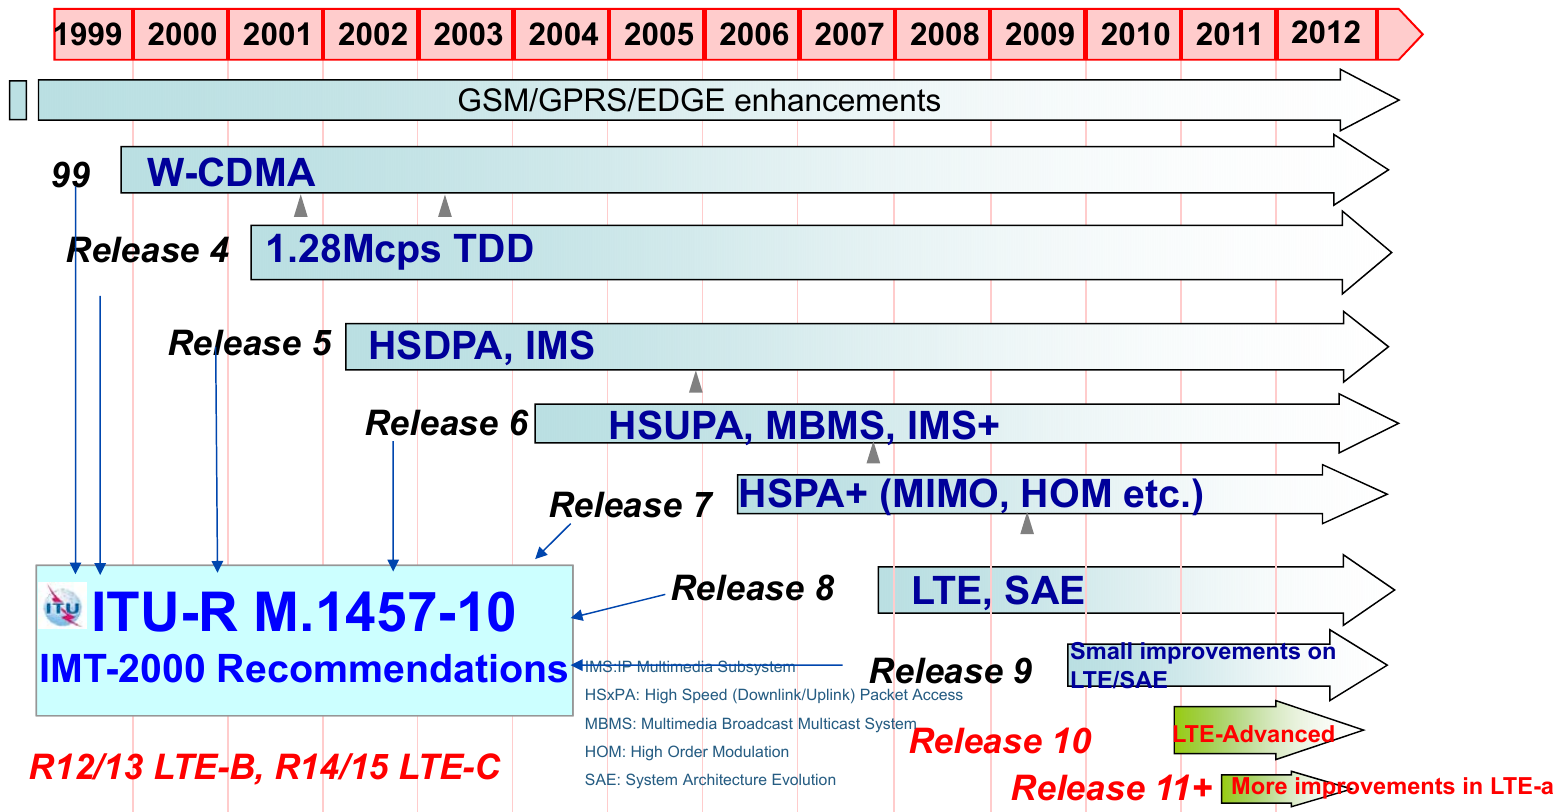
\includegraphics[
		width=14cm,
		%height=15cm
	]{images/Tema 4/LTE standardization.png}
	\caption{
		\label{fig:unit4_LTE_stand}
		LTE standardization
	}
\end{figure}

\subsection{Description}

\subsubsection{Architecture}

LTE defines new elements for its implementation:
\begin{itemize}
	\item {
		Evolved UTRAN (E-UTRAN): Its a new network whose functionality is simmilar to UTRAN in UMTS. Some of its elements are:
		\begin{itemize}
			\item {
				Evolved Node B: Theri roles are similar to Node B in UMTS. These are:
				\begin{itemize}
					\item Radio resource managements.
					\item Synchronization and interference management.
					\item IP header compression.
					\item Ciphering and integrity protection for user data.
					\item MME selection.
					\item Routing from or to S-GW.
				\end{itemize}
			}
			\item Interface: It provides handovers, load balance and interference cancellation.
		\end{itemize}
	}
	\item {
		Evolved Packet Core (EPC): Its a new network whose functionality is simmilar to Core Network in UMTS. Some of its elements are:
		\begin{itemize}
			\item {
				Mobile Management Entity (MME):
				\begin{itemize}
					\item Access Security Control (AS).
					\item Signaling and security in Non Stratum Access (NAS) between Core and terminal.
					\item Tracking and paging area management.
					\item S-GW and P-GW selection.
					\item Roaming and authentication.
					\item Flow control EPS (tunnel, EPS bearer).
				\end{itemize}
			}
			\item {
				Serving Gateway (S-GW):
				\begin{itemize}
					\item Packets routing.
					\item QoS at transport level for DiffServ.
					\item UE only associated to one SW in time.
				\end{itemize}
			}
			\item {
				Packet Dana Network Gateway (P-GW):
				\begin{itemize}
					\item IP Address for UE.
					\item QoS at transport level.
					\item Anchorage for mobility at the user plane.
					\item Packets filtering.
				\end{itemize}
				\begin{figure}[H]
					\centering
					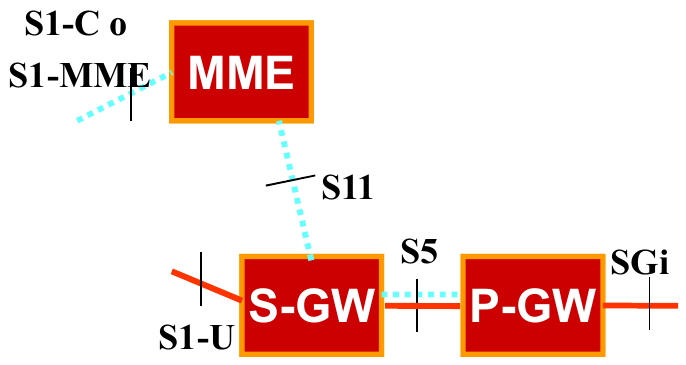
\includegraphics[
						width=8cm,
						%height=15cm
					]{images/Tema 4/EPC 1.png}
					\caption{
						\label{fig:unit4_LTE_EPC1}
						EPC 1
					}
				\end{figure}
			}
			\item {
				Home Subscriber Server (HSS):
				\begin{itemize}
					\item User data and user management logic.
					\item {
						Subscriber data from users:
						\begin{itemize}
							\item Authentication and authorization credantials for access.
							\item Information of mobility management in LTE and among other LTE networks.
						\end{itemize}
					}
					\item Access networks.
					\item S6a interface.
				\end{itemize}
			}
			\item {
				Policy and Charging Rules Function (PCRF):
				\begin{itemize}
					\item Billing control.
					\item Policies for traffic control. QoS management and service authorization.
					\item Applied to Policy and Charging Enforcement Function (PCEF).
				\end{itemize}
			}
			\item {
				Equipment Identity Register (EIR):
				\begin{itemize}
					\item Database with devices information.
					\item Stolen devices can not access to the network.
					\item S13 interface.
				\end{itemize}
				\begin{figure}[H]
					\centering
					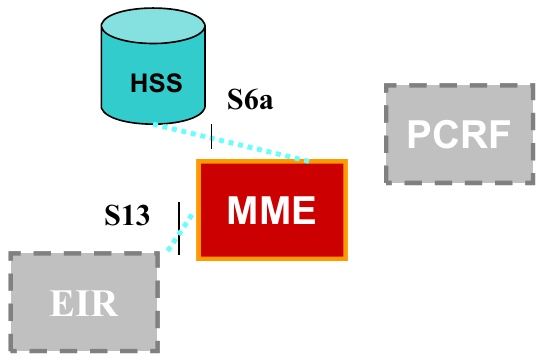
\includegraphics[
						width=8cm,
						%height=15cm
					]{images/Tema 4/EPC 2.png}
					\caption{
						\label{fig:unit4_LTE_EPC2}
						EPC 2
					}
				\end{figure}
			}
		\end{itemize}
	}
\end{itemize}

\begin{figure}[H]
	\centering
	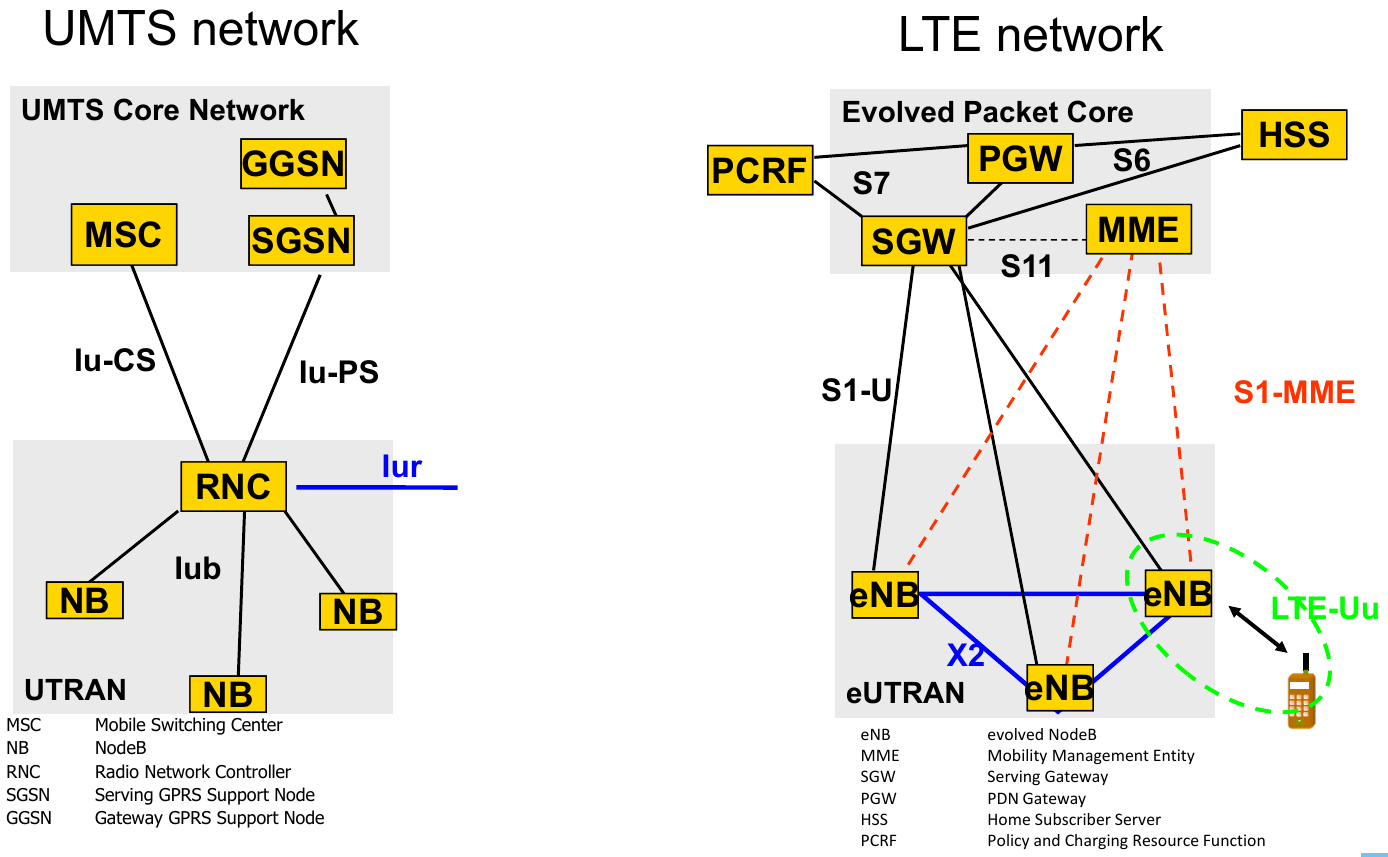
\includegraphics[
		width=14cm,
		%height=15cm
	]{images/Tema 4/UMTS vs LTE architecture.png}
	\caption{
		\label{fig:unit4_UMTS_vs_LTE}
		UMTS vs LTE architecture
	}
\end{figure}

\subsubsection{General characteristics}

LTE is designed to do not reserve fixed resources to any user. There are only common shared channels instead of dedicated ones as in UMTS.

Used modulation:
\begin{itemize}
	\item UL: SC-FDMA. Low Peak to Average Power Ratio (PAPR) and orthogonality in frequency among users.
	\item DL: OFDMA. Robust against multipath, flexibility, advanced signal processing techniques.
\end{itemize}

Constellations:
\begin{itemize}
	\item UL: QPSK, 16QAM and 64QAM (optional) for data and control, except PRACH, that uses phase sequences Zadoff-Chu.
	\item DL: QPSK, 16QAM and 64QAM for data. BPSK and QPSK for control.
\end{itemize}

Bandwidth for both UL and DL goes from 0 to 20 MHz in steps of 180 kHz (12 subcarriers x 15 kHz/subcarrier). In practice: 1.4 (6 RB), 3 (15 RB) , 5 (25 RB), 10 (50 RB), 15 (75 RB) and 20 (100 RB) MHz. Also 7.5 kHz in Multicast Broadcast Single Frequency Networks (MBSFN).
\begin{figure}[H]
	\centering
	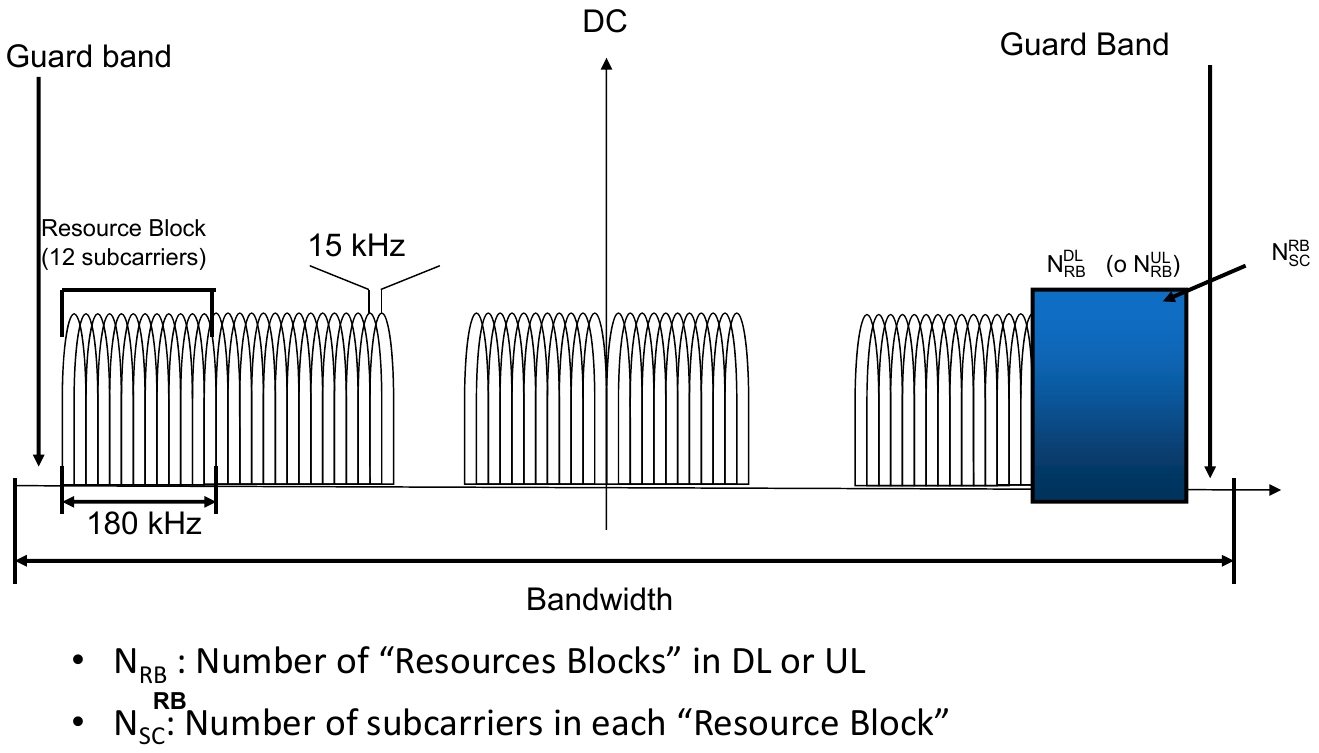
\includegraphics[
		width=14cm,
		%height=15cm
	]{images/Tema 4/LTE bandwidth.png}
	\caption{
		\label{fig:unit4_LTE_BW}
		LTE bandwidth
	}
\end{figure}

There is no macro diversity as in UMTS. Handover is hard due to OFDM.

Protocol architecture is simple since it is based on shared channels and only packet domain and VoIP. Network architecture is also simple:
\begin{itemize}
	\item Only eNodeB
	\item {
		Few interfaces in Radio Access Network (RAN):
		\begin{itemize}
			\item eNodeB $\rightarrow$ MME/SAE-Gateway (S1)
			\item eNodeB $\rightarrow$ eNodeB (X2)
		\end{itemize}
	}
\end{itemize}

LTE manages a resources Grid (T-F):
\begin{itemize}
	\item 1 frame is 10ms. It has 10 subframes.
	\item 1 subframe is 1ms. It has 2 slots.
	\item 1 slot is 0.5ms and has Nsymb symbols.
	\item 1 ``resource element'' is one subcarrier and one symbol.
	\item 1 ``resource block'' is 0.5 ms and has 12 subcarriers per OFDM symbol.
	\item {
		There are NRB ``resource blocks'':

		$6 < NRB < 110$
	}
\end{itemize}

\begin{figure}[H]
	\centering
	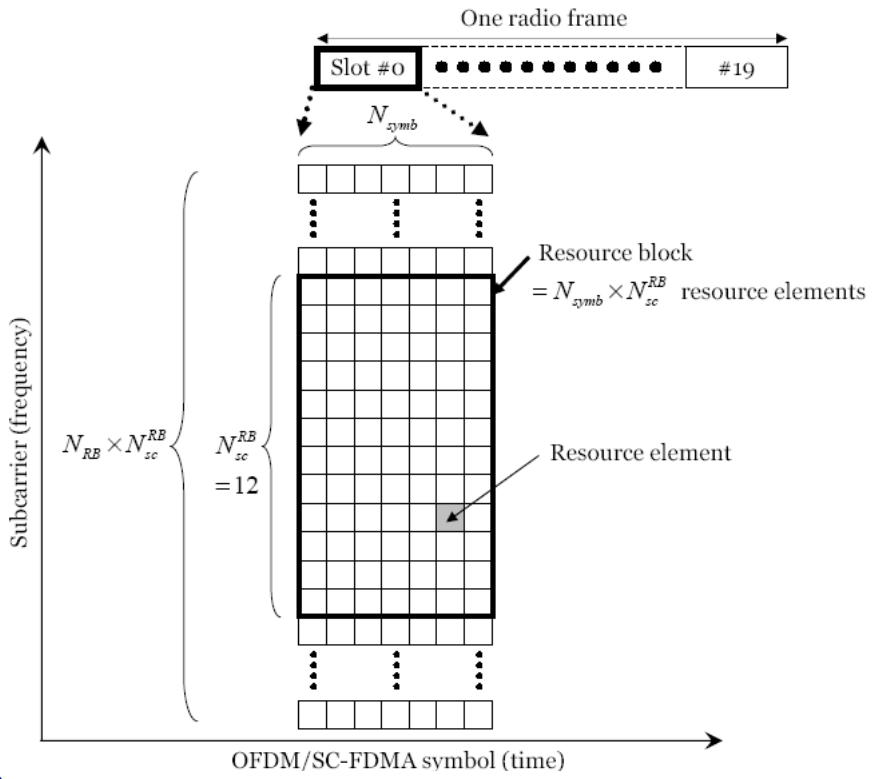
\includegraphics[
		width=14cm,
		%height=15cm
	]{images/Tema 4/LTE resources grid.png}
	\caption{
		\label{fig:unit4_LTE_resources_grid}
		LTE resources grid
	}
\end{figure}

For resource and assignations:
\begin{itemize}
	\item Resource Element (RE): 1 element in the T-F grid. Fundamental element (smallest) for control.
	\item {
		Resource Block (RB): Minimum amount of resource that can be allocated for a user (12 subcarriers x 1 slot). We can consider:
		\begin{itemize}
			\item Physical Resource Block (PRB): 180 kHz x 0.5 ms.
			\item {
				Virtual Resource Block (VRB):
				\begin{itemize}
					\item Localized.
					\item Distributed.
				\end{itemize}
			}
			\item Resource Block Group (RBG): Group of assigned RB to a user.
		\end{itemize}
	}
\end{itemize}

\subsection{Physical channels}

LTE uses several physical channels for downlink:
\begin{itemize}
	\item Physical Broadcast Channel (PBCH).
	\item Physical Downlink Shared Channel (PDSCH).
	\item Physical Control Format Indicator Channel (PCFICH).
	\item Physical Downlink Control Channel (PDCCH).
	\item Physical HARQ Indicator Channel (PHICH).
	\item Physical Multicast Channel (PMCH).
\end{itemize}

\begin{figure}[H]
	\centering
	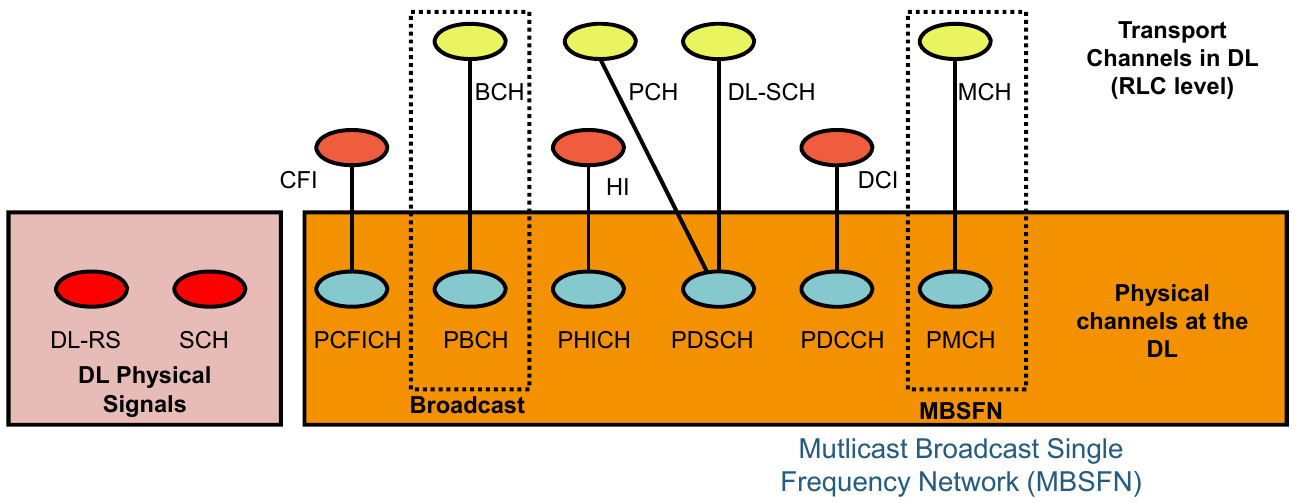
\includegraphics[
		width=14cm,
		%height=15cm
	]{images/Tema 4/LTE physical channels - Downlink.png}
	\caption{
		\label{fig:unit4_LTE_phys_down}
		LTE physical channels for downlink
	}
\end{figure}

And for uplink:
\begin{itemize}
	\item Physical Random Access Channel (PRACH).
	\item Physical Uplink Control Channel (PUCCH).
	\item Physical Uplink Shared Channel (PUSCH).
\end{itemize}

\begin{figure}[H]
	\centering
	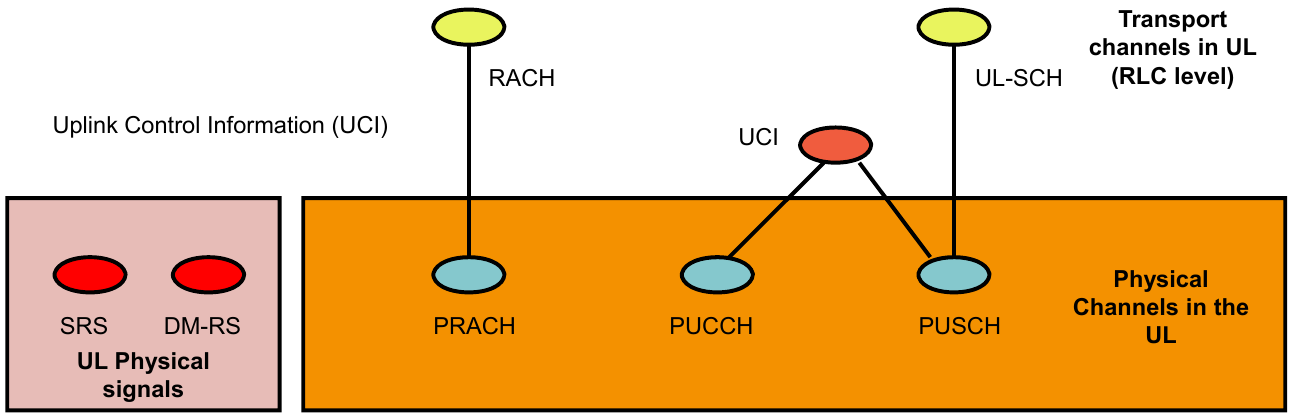
\includegraphics[
		width=14cm,
		%height=15cm
	]{images/Tema 4/LTE physical channels - Upwnlink.png}
	\caption{
		\label{fig:unit4_LTE_phys_up}
		LTE physical channels for uplink
	}
\end{figure}

It also uses signals for for uplink:
\begin{itemize}
	\item Sounding Reference Signal (SRS).
	\item Demodulation Reference Signal (DM-RS).
\end{itemize}

\subsection{Key features}

\subsubsection{In LTE Advanced (LTE-A)}

A wider bandwidth is supported through carrier aggregation:
\begin{itemize}
	\item Use of multiple component carriers(CC) to extend bandwidth up to 100 MHz.
	\item Common physical layer parameters between component carrier and LTE Rel-8 carrier.
	\item Improvement of peak data rate, backward compatibility with LTE Rel-8.
\end{itemize}

\begin{figure}[H]
	\centering
	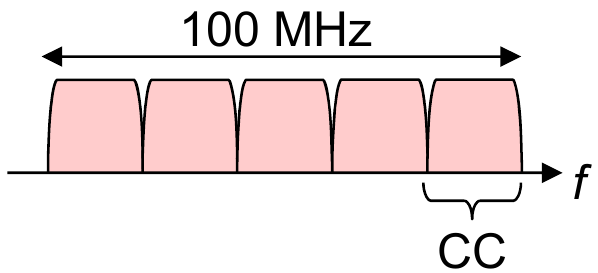
\includegraphics[
		width=6cm,
		%height=15cm
	]{images/Tema 4/LTE carrier aggregation.png}
	\caption{
		\label{fig:unit4_LTE_carrier_aggregation}
		LTE carrier aggregation
	}
\end{figure}

Advanced MIMO techniques are used:
\begin{itemize}
	\item Extension to up to 8-layer transmission in downlink.
	\item Introduction of single-user MIMO up to 4-layer transmission in uplink.
	\item Enhancements of multi-user MIMO.
	\item Improvement of peak data rate and capacity.
\end{itemize}

\begin{figure}[H]
	\centering
	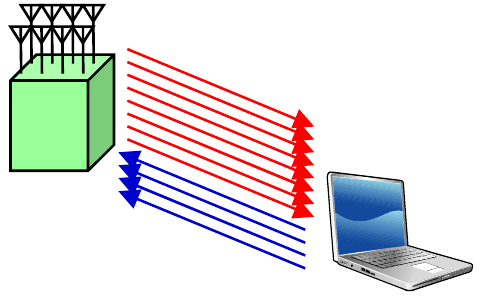
\includegraphics[
		width=5cm,
		%height=15cm
	]{images/Tema 4/LTE MIMO.png}
	\caption{
		\label{fig:unit4_LTE_MIMO}
		LTE MIMO
	}
\end{figure}

Heterogeneous network and enhanced Inter-Cell Interference Coordination (eICIC):
\begin{itemize}
	\item Interference coordination for overlaid deployment of cells with different transmission power.
	\item Improvement of cell-edge throughput and coverage.
\end{itemize}

\begin{figure}[H]
	\centering
	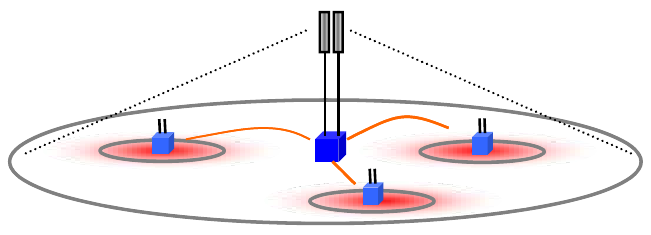
\includegraphics[
		width=8cm,
		%height=15cm
	]{images/Tema 4/LTE eCIC.png}
	\caption{
		\label{fig:unit4_LTE_eCIC}
		LTE eCIC
	}
\end{figure}

Relay:
\begin{itemize}
	\item Type 1 relay supports radio backhaul and creates a separate cell and appear as Rel. 8 LTE eNB to Rel. 8UEs.
	\item Improvement of coverage and flexibility of service area extension.
\end{itemize}

\begin{figure}[H]
	\centering
	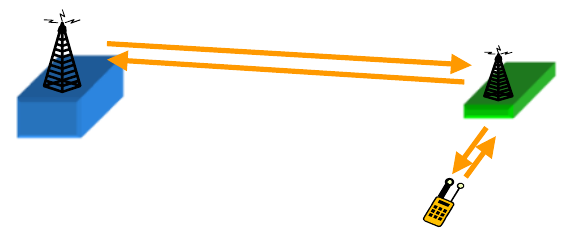
\includegraphics[
		width=8cm,
		%height=15cm
	]{images/Tema 4/LTE relay.png}
	\caption{
		\label{fig:unit4_LTE_relay}
		LTE relay
	}
\end{figure}

Coordinated Multi-Point transmission and reception (CoMP):
\begin{itemize}
	\item Support of multi-cell transmission and reception.
	\item Improvement of cell-edge throughput and coverage.
\end{itemize}

\begin{figure}[H]
	\centering
	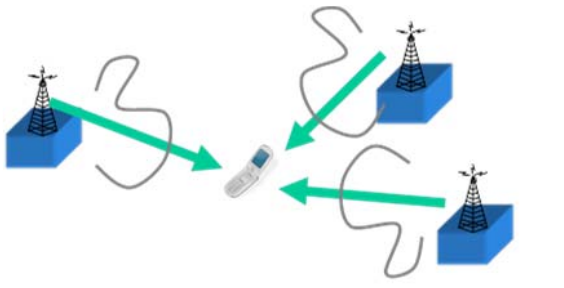
\includegraphics[
		width=8cm,
		%height=15cm
	]{images/Tema 4/LTE CoMP.png}
	\caption{
		\label{fig:unit4_LTE_CoMP}
		LTE CoMP
	}
\end{figure}

\subsubsection{In LTE-B physical layer}

There are some improvements in local area access:
\begin{itemize}
	\item More heteregoneous and complementary access technologies.
	\item Soft cells.
	\item Dynamic TDD in pico cells.
\end{itemize}

There are also improvements in energy efficiency and M2M communicatons.

There are general improvements in physical layer:
\begin{itemize}
	\item In beamforming.
	\item CoMP.
	\item Receivers.
	\item More bands (< 3 GHz).
	\item Deployment density increasing.
\end{itemize}

\section{Femtocells}

\subsection{Introduction}

Femtocells are small base station used to extend mobile coverage to inner spaces. It is connected to network through DSL or wire. In UMTS, it equals to a node B station.

\begin{figure}[H]
	\centering
	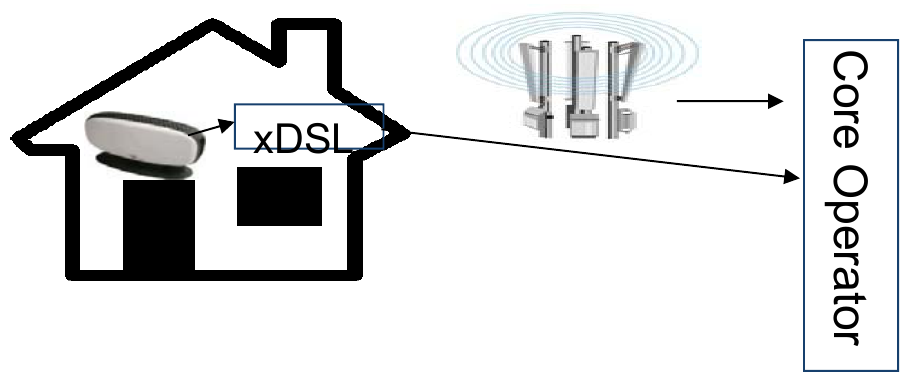
\includegraphics[
		width=10cm,
		%height=15cm
	]{images/Tema 4/Femtocells.png}
	\caption{
		\label{fig:unit4_Femtocells}
		Femtocells
	}
\end{figure}

\subsection{Benefits}

Their benefits to operators are:
\begin{itemize}
	\item They improve network coverage.
	\item They reduce backhaul cost (low dimensions, low energy consumption, \ldots).
	\item They increase subscribers capacity.
	\item They improve customer retention.
	\item They increase revenue opportunities since tnew applications).
	\item They address the VoIP threat.
	\item They stimulate 3G usage.
\end{itemize}

Their benefits to customers are:
\begin{itemize}
	\item They reduce domestic telephone call charges.
	\item They improve indoor coverage.
	\item They improved broadband experience.
	\item They work with existing handsets.
	\item They reduce mobile battery drain.
	\item They offer new converged services.
	\item One consolidated bill.
\end{itemize}

\subsection{Problems and challenges}

Main problems and challenges include:
\begin{itemize}
	\item Interference.
	\item QoS.
	\item Security.
	\item Emergency calls.
\end{itemize}

\section{5G and New Radio (NR)}

\subsection{Introduction}

5G is the name for the incoming fifth generation of mobile communications. It will be based on standard IEEE 802.11ac and will focus on a set of goals:
\begin{itemize}
	\item User quality of experience.
	\item System performance.
	\item Improvements on services.
	\item Business model.
	\item Operation and maintenance.
\end{itemize}

It supposes a smooth evolution from 4G. At the beginning, the Radio Nodes (RN) will be handled by 4G controllers. Some evolutions will appear the so-called 4.9G.

\begin{figure}[H]
	\centering
	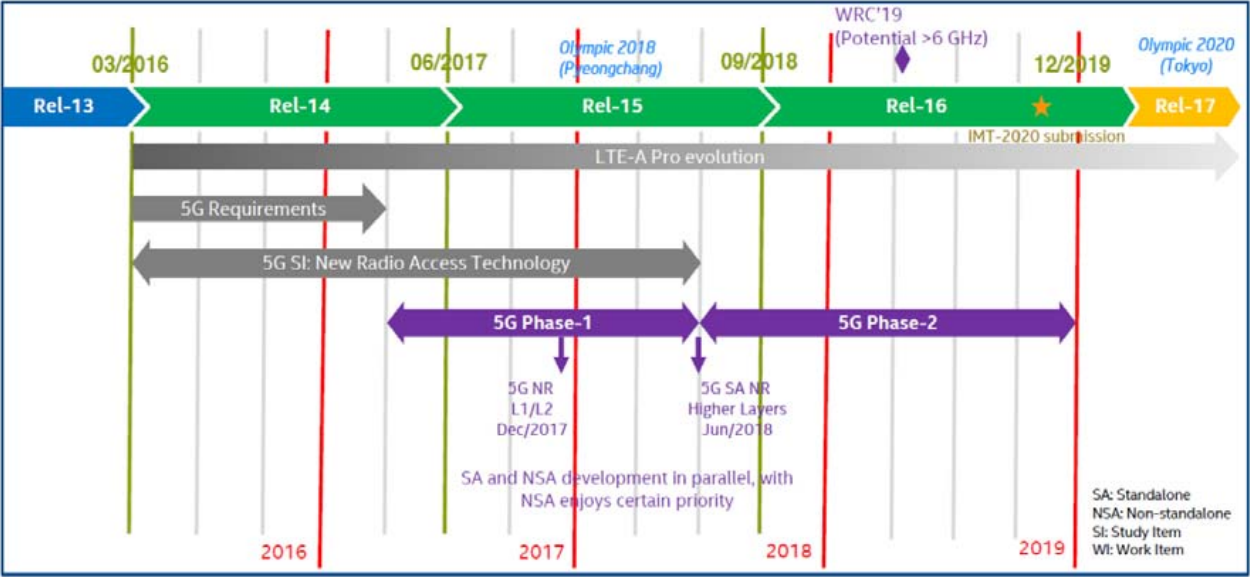
\includegraphics[
		width=14cm,
		%height=15cm
	]{images/Tema 4/4G - 5G.png}
	\caption{
		\label{fig:unit4_4G_5G}
		4G - 5G
	}
\end{figure}

\subsection{Description}

Minimum specifications for 5G are described by ITU on IMT-2020 standard:
\begin{itemize}
	\item 100 MHz of bandwidth, up to 1 GHz (above 6 Ghz).
	\item Download Peak Rate of 20 Gbps.
	\item Uplink Peak Rate of 10 Gbps.
	\item Downlink Peak Spectral Efficiency of 30 bps/Hz.
	\item Uplink Peak Spectral Efficiency of 15 bps/Hz.
	\item Downlink User Experienced data rate of 100 Mbps.
	\item Uplink User Experienced data rate of 50 Mbps.
\end{itemize}

\begin{figure}[H]
	\centering
	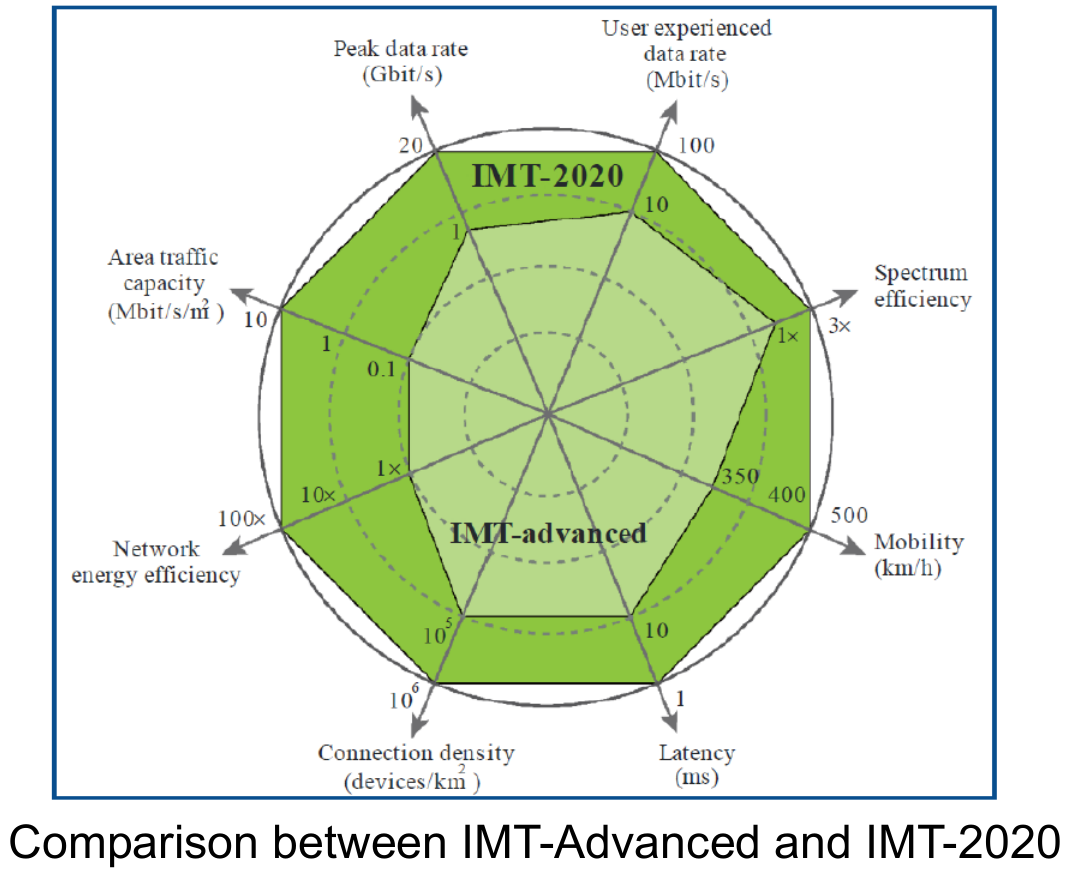
\includegraphics[
		width=14cm,
		%height=15cm
	]{images/Tema 4/Comparison between IMT-Advanced and IMT-2020.png}
	\caption{
		\label{fig:unit4_comparison_ad_2020}
		Comparison between IMT-Advanced and IMT-2020
	}
\end{figure}

It also includes the definition of New Radio (NR).

5G also introduces new communications paradigms:
\begin{itemize}
	\item Massive Machine Type Communications (mMTC): A lot of connected devices (IoE, wearable, smart buildings, \ldots).
	\item Enhanced Mobile Broadband (eMBB): High data rate and quality of service, even at cell edges (streaming, augmented reality, \ldots).
	\item Ultra-reliable and Low Latency Communications (uRLLC): High reliability and low latency (traffic, health, games, \ldots).
\end{itemize}

\begin{figure}[H]
	\centering
	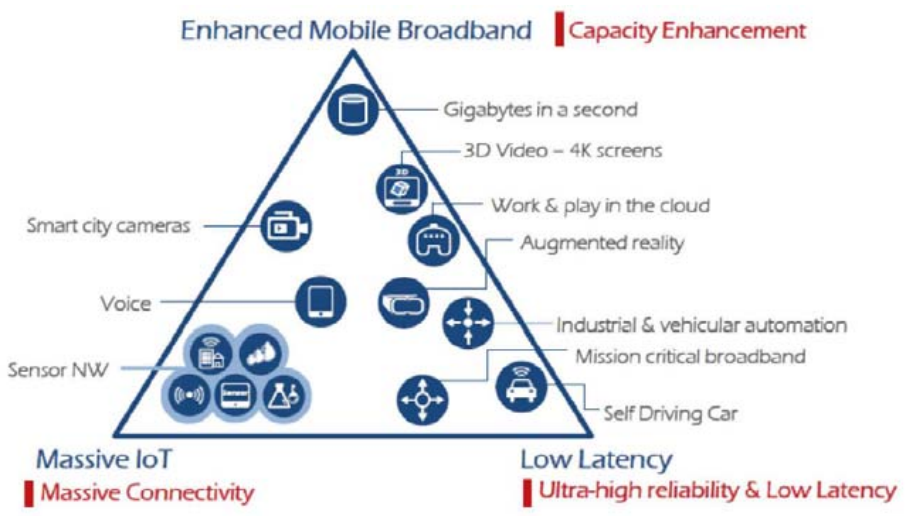
\includegraphics[
		width=8cm,
		%height=15cm
	]{images/Tema 4/5G paradigms.png}
	\caption{
		\label{fig:unit4_5G_paradigms}
		5G paradigms
	}
\end{figure}

\subsection{Technologies}

Different technologies are being analyzed:
\begin{itemize}
	\item Millimeter waves: Frequencies much higer than 6 GHz. Beamforming mandatory.
	\item Massive MIMO: Lots of antennas.
	\item Full Duplex: Improvements in efficiency.
	\item Non Orthogonal Multiple Access (NOMA): By using codes.
	\item 256QAM: In 4G, up to 64QAM.
	\item New waveforms.
	\item {
		New network architectures: Software Defined Network (SDN) and Network Functions Virtualization (NFV).
		\begin{figure}[H]
			\centering
			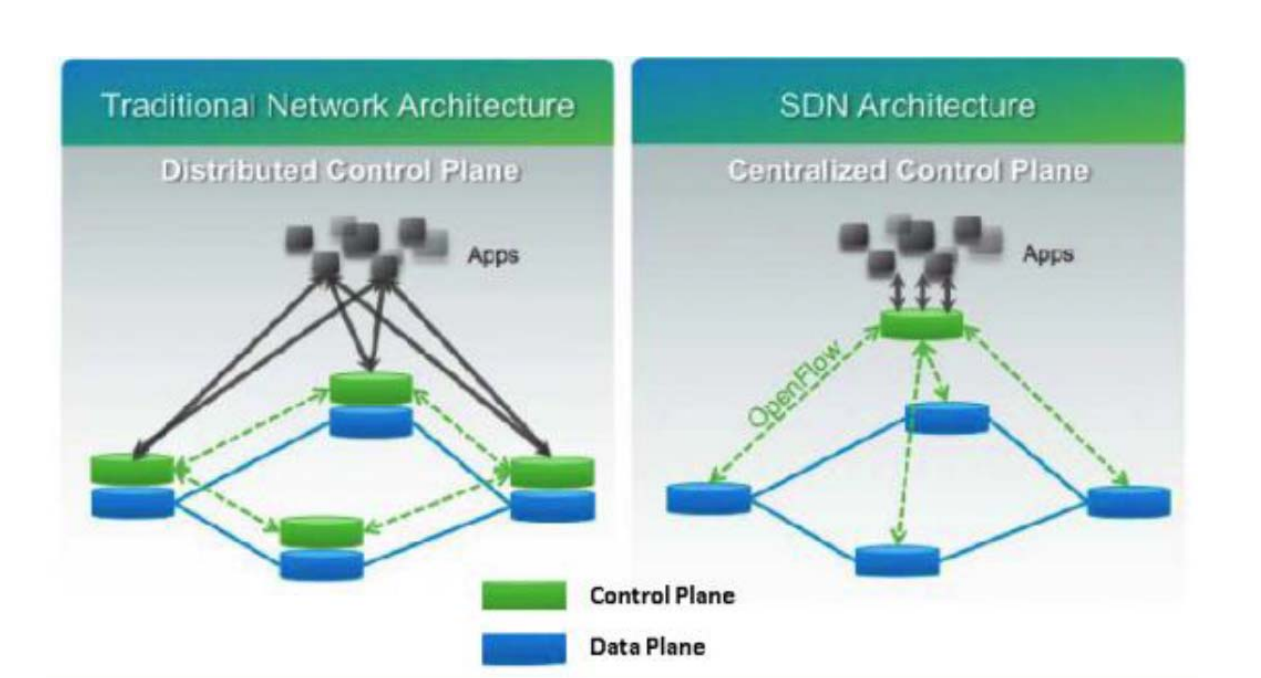
\includegraphics[
				width=14cm,
				%height=15cm
			]{images/Tema 4/5G network architectures.png}
			\caption{
				\label{fig:unit4_5G_net_arch}
				5G network architectures
			}
		\end{figure}
	}
	\item {
		CloudRAN: RAN with central controller.
		\begin{figure}[H]
			\centering
			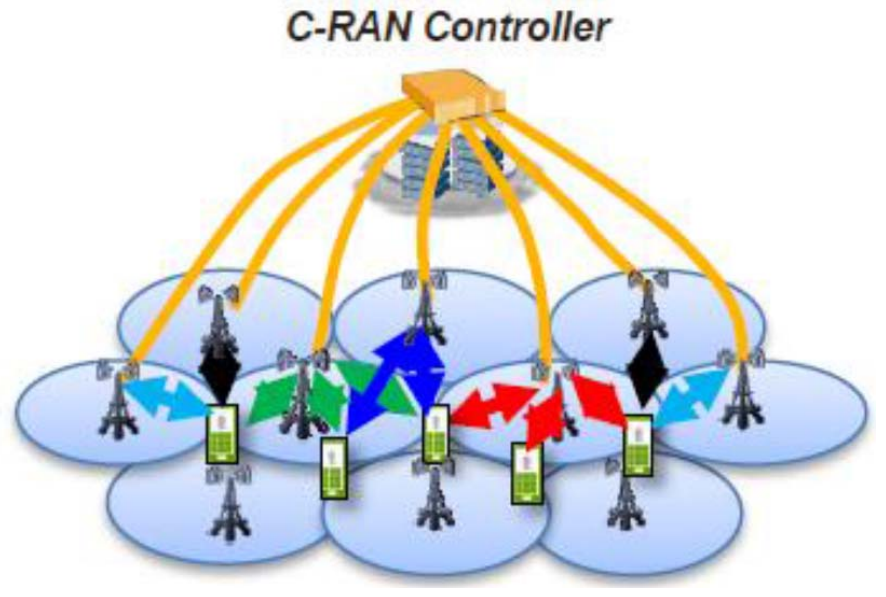
\includegraphics[
				width=8cm,
				%height=15cm
			]{images/Tema 4/CloudRAN.png}
			\caption{
				\label{fig:unit4_5G_CloudRAN}
				CloudRAN
			}
		\end{figure}
	}
\end{itemize}



\end{document}
